% ---
% Capitulo de Desenvolvimento da Aplicação
% ---
\chapter{Desenvolvimento}
% ---
Este capítulo apresenta a solução de \textit{Business Intelligence} do Setor de Nutrição Clínica do HU-UFS abordando estratégias, necessidades informacionais e peculiaridades do setor de nutrição do hospital. Serão descritas as atividades de criação do modelo relacional do \textit{Data Warehouse}, detalhamento do processo de ETL e a elaboração da interface OLAP. São apresentados também a interface web destinada aos tomadores de decisão, os resultados das consultas OLAP e informações referentes ao escopo do projeto e ao HU-UFS.
% ---
\section{Hospital Universitário de Aracaju - HU-UFS}
% ---
O Hospital Universitário (HU) é um campus da Universidade Federal de Sergipe (UFS) desde 1984, funcionando como centro hospitalar de assistência, ensino e pesquisa em ciências da saúde. Atualmente, o HU-UFS em Sergipe ocupa um espaço de referência e excelência na prestação de assistência médico-hospitalar de média e alta complexidade \cite{sitehuufs}.

Em 2013, a UFS e a Empresa Brasileira de Serviços Hospitalares (EBSERH) firmaram convênio para transferência da administração do HU no âmbito do Programa Nacional de Reestruturação dos Hospitais Universitários Federais (REHUF). O HU-UFS tornou-se a nona filial da EBSERH com administração vigorosa em todas as áreas do hospital. Em abril de 2016, o HU-UFS tornou-se habilitado para o atendimento especializado de pessoas com deficiência auditiva, bem como, para procedimentos de vasectomia. Atualmente, a estrutura do hospital inclui departamentos de Clínica Médica, Clínica Cirúrgica, Pediatria, Unidade de Terapia Intensiva (UTI) e Centro Cirúrgico. Vários cursos de graduação, pós-graduação, residência médica e multiprofissional utilizam as instalações desse hospital-escola para desenvolver práticas e pesquisas inovadoras \cite{sitehuufs}. 

% ---
\section{Escopo do Projeto}
% ---
A Unidade de Nutrição Clínica do HU armazena seus registros de formulários de acompanhamento nutricional dos pacientes em planilhas eletrônicas. As informações entregues à gestão do hospital são consultadas nestas planilhas pela chefia do setor. Os dados mais relevantes para a chefia estão relacionadas aos índices de classificação de risco, estado nutricional, utilização de suplementação e utilização de dietas enterais e suas relações com possíveis complicações identificadas nos pacientes internados nas diversas clínicas do hospital. Um dos formulários utilizados para coleta de dados básicos para essas planilhas é apresentado na \autoref{fig_figuraFormularioDiagClinicoNutri}.

\begin{figure}[htb]
	\caption{\label{fig_figuraFormularioDiagClinicoNutri}Formulário de Diagnóstico Clínico-Nutricional.}
	\begin{center}
	    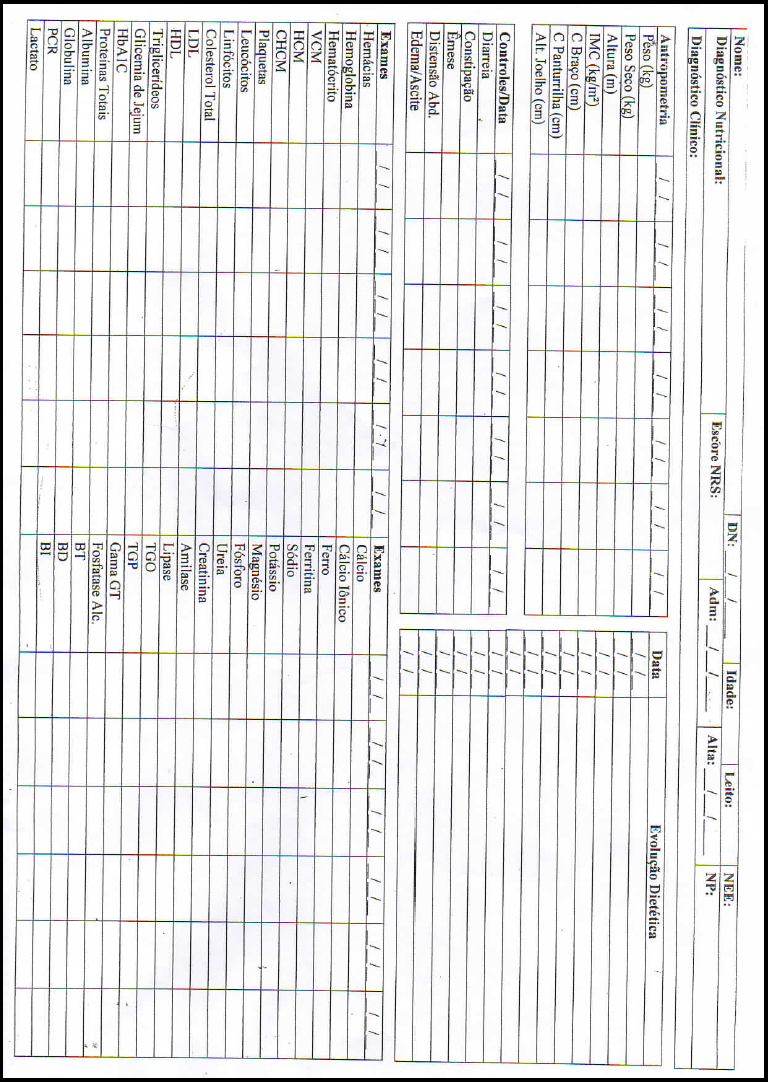
\includegraphics[scale=0.569]{Imagens/figura - formulario diagnostico clinico nutricional.png}
	\end{center}
	\legend{Fonte: \cite{huufs}.}
\end{figure}

Todos esses dados, antes de serem carregados no \textit{Data Warehouse} passaram por um processo de ETL, que de forma sistemática realiza tratamento e limpeza dos dados advindos dos diversos arquivos fornecidos pela unidade de nutrição e pelo hospital. 

Um ponto importante a ser considerado, é que devido ao surto mundial de Sars-Cov-2, confirmado pela \citeonline{whocovid} em 2020, vários hospitais tiveram de passar por revisões dos seus protocolos de atendimento. Com a emissão de resolução do Conselho Federal de Nutrição e do Protocolo Operacional Padrão emitido pelo HU-UFS, a Unidade de Nutrição não mais realizou triagens nutricionais em pacientes de forma presencial e o acompanhamento nutricional foi realizado apenas de forma online e com regras diferentes para avaliação \cite{protocolocovidnutri, cfnutri646}. Com todas as mudanças ocorridas em 2020, a unidade não foi capaz de realizar o registro de alguns dados conforme padrão de anos anteriores e disponibilizou apenas a fonte de dados do ano de 2019 para este trabalho.

Com os dados disponíveis carregados no DW foi necessário criar um modelo de dados OLAP, no qual as informações são organizadas conceitualmente em cubos de dados para análise dinâmica e multidimensional dos dados consolidados.

Com a possibilidade de consultas dinâmicas oferecidas pelo OLAP a Unidade de Nutrição Clínica solicitou além dos dados quantitativos também gráficos de comparação, composição e tendência para diferentes dimensões, sempre considerando uma visão de todo o hospital e uma visão por enfermaria como descritos abaixo: 

Para o indicador de Triagem Nutricional Realizada, as seguintes informações foram solicitados:
\begin{itemize}
    \item Quantidade de Triagens Nutricionais Realizadas ao ano;
    \item Quantidade de Triagens Nutricionais Realizadas por mês;
    \item Quantidade de Triagens Nutricionais Realizadas por Enfermaria ao ano;
    \item Tendência de Triagens Nutricionais Realizadas por Enfermaria.
\end{itemize}

Para o indicador de Classificação de Risco foram solicitadas as seguintes informações:
\begin{itemize}
    \item Percentual de Pacientes segundo Classificação de Risco ao ano;
    \item Percentual de Pacientes segundo Classificação de Risco detalhado por mês;
    \item Percentual de Pacientes segundo Classificação de Risco por Enfermaria ao ano;
    \item Tendência de Pacientes segundo Classificação de Risco por Enfermaria detalhado por mês.
\end{itemize}

Para o indicador de Estado Nutricional foram solicitadas as seguintes informações:
\begin{itemize}
    \item Percentual de Pacientes segundo Estado Nutricional ao ano;
    \item Percentual de Pacientes segundo Estado Nutricional detalhado por mês;
    \item Percentual de Pacientes segundo Estado Nutricional por Enfermaria ao ano;
    \item Tendência de Pacientes segundo Estado Nutricional por Enfermaria detalhado por mês.
\end{itemize}

Para o indicador de Uso de Suplementação foram solicitadas as seguintes informações:
\begin{itemize}
    \item Quantidade de Pacientes em Uso de Suplemento;
    \item Quantidade de Pacientes em Uso de Suplemento por Enfermaria;
    \item Percentual de Pacientes segundo Uso de Suplementação ao ano;
    \item Percentual de Pacientes segundo Uso de Suplementação por Enfermaria ao ano;
    \item Tendência de Pacientes segundo Uso de Suplementação por Enfermaria detalhado por mês;
    \item Comparativo de pacientes que utilizam Suplementação com média de dias internado;
    \item Comparativo de pacientes que utilizam Suplementação com média de dias internado por enfermaria.
\end{itemize}

Para o indicador de Insumo foi solicitada a seguinte informação:
\begin{itemize}
    \item Percentual de Insumos utilizados por Enfermaria.
\end{itemize}

Para o indicador de Uso de Dieta Enteral foram solicitadas as seguintes informações:
\begin{itemize}
    \item Quantidade de Pacientes em Uso de Dieta Enteral;
    \item Quantidade de Pacientes em Uso de Dieta Enteral por Enfermaria;
    \item Percentual de Pacientes segundo Uso de Dieta Enteral ao ano;
    \item Percentual de Pacientes segundo Uso de Dieta Enteral por Enfermaria ao ano;
    \item Tendência de Pacientes segundo Uso de Dieta Enteral por Enfermaria detalhado por mês;
    \item Comparativo de pacientes que utilizam Dieta Enteral com média de dias internado;
    \item Comparativo de pacientes que utilizam Dieta Enteral com média de dias internado por enfermaria.
\end{itemize}

Para o indicador de Complicações, que podem ocorrer por Uso de Suplementação e Uso de Dieta Enteral foram solicitadas as seguintes informações:
\begin{itemize}
    \item Percentual de Complicações em Uso de Suplementação ao ano;
    \item Percentual de Complicações em Uso de Suplementação por Enfermaria ao ano;
    \item Percentual de Complicações em Uso de Dieta Enteral ao ano;
    \item Percentual de Complicações em Uso de Dieta Enteral por Enfermaria ao ano.
\end{itemize}

Para o indicador de Desfecho onde podem ocorrer altas, transferências ou óbitos, combinado a Dimensão de Classificações de Risco foram solicitadas as seguintes informações:
\begin{itemize}
    \item Percentual de Desfecho por Classificação de Risco ao ano;
    \item Percentual de Desfecho por Classificação de Risco por Enfermaria ao ano.
\end{itemize}

\section{Solução de \textit{Business Intelligence}}

A solução BI desenvolvida utilizou o conjunto de ferramentas \textit{Pentaho Community}, que são mantidas e disponibilizadas gratuitamente pela Hitachi Vantara©. O \textit{Pentaho Community} fornece um pacote de ferramentas completo para soluções BI. Para este trabalho foram utilizadas as seguintes ferramentas: \textit{Pentaho Data Integration, Pentaho Schema Workbench e Pentaho Business Analytics Platform}.

Alguns pré-requisitos são necessários para o bom funcionamento do ambiente. Foram instalados os seguintes \textit{softwares} auxiliares: Java SE \textit{Runtime Environment} 8 \textit{update} 261, PostgreSQL 12.5, PG Admin 4.24 e SQL \textit{Power Arquitect} 1.0.8. Ainda nesta seção são descritas as etapas de modelagem multidimensional do \textit{Data Warehouse} e do \textit{Data Mart}, o processo de ETL, o mapeamento lógico do cubo de dados OLAP, as consultas e os resultados dos \textit{Dashboards}.

\subsection{Modelagem Multidimensional}
Ao analisar as características das informações solicitadas pela gestão da unidade de nutrição, considerando cada necessidade como um problema a ser resolvido, foi elaborado o modelo multidimensional usando a estrutura \textit{star schema}. O esquema foi modelado com 13 dimensões (Hospital, Enfermaria, Tempo, Paciente, Classificação Nutricional, Estado Nutricional, Complicações, Triagem Realizada, Suplementação, Dieta Enteral, Insumos, Edema e Desfecho) e uma Fato (Nutrição). A \autoref{fig_modelagemdatawarehouse} mostra o modelo de dados do \textit{Data Warehouse} projetado neste trabalho.

\begin{figure}[htb]
	\caption{\label{fig_modelagemdatawarehouse}Modelo Multidimensional do \textit{Data Warehouse.}}
	\begin{center}
	    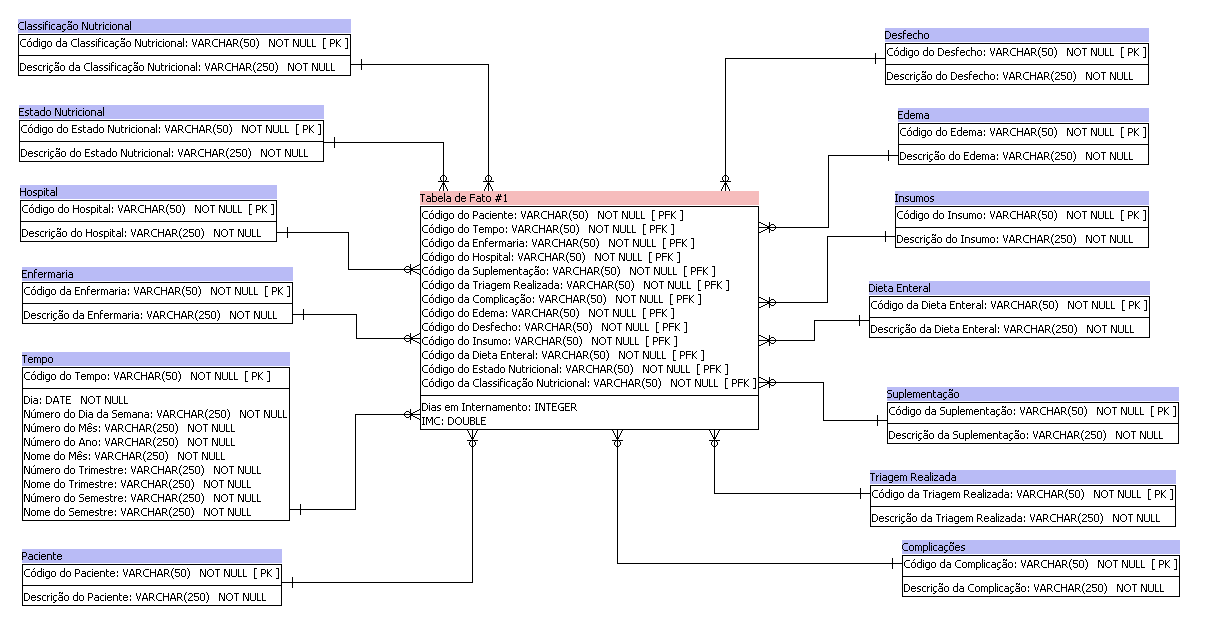
\includegraphics[scale=0.53]{Imagens/figura - modelagem multidimensional datawarehouse.png}
	\end{center}
	\legend{Fonte: Autor.}
\end{figure}

\newpage
Com o objetivo de permitir melhor performance para as consultas também foi projetado um cubo OLAP de modelo relacional, mais especificamente chamado de \textit{Relational Online Analitycal Processing} (ROLAP), como é mostrado na \autoref{fig_modelagemdatamart}.

\begin{figure}[htb]
	\caption{\label{fig_modelagemdatamart}Modelo Relacional do \textit{Data Mart}.}
	\begin{center}
	    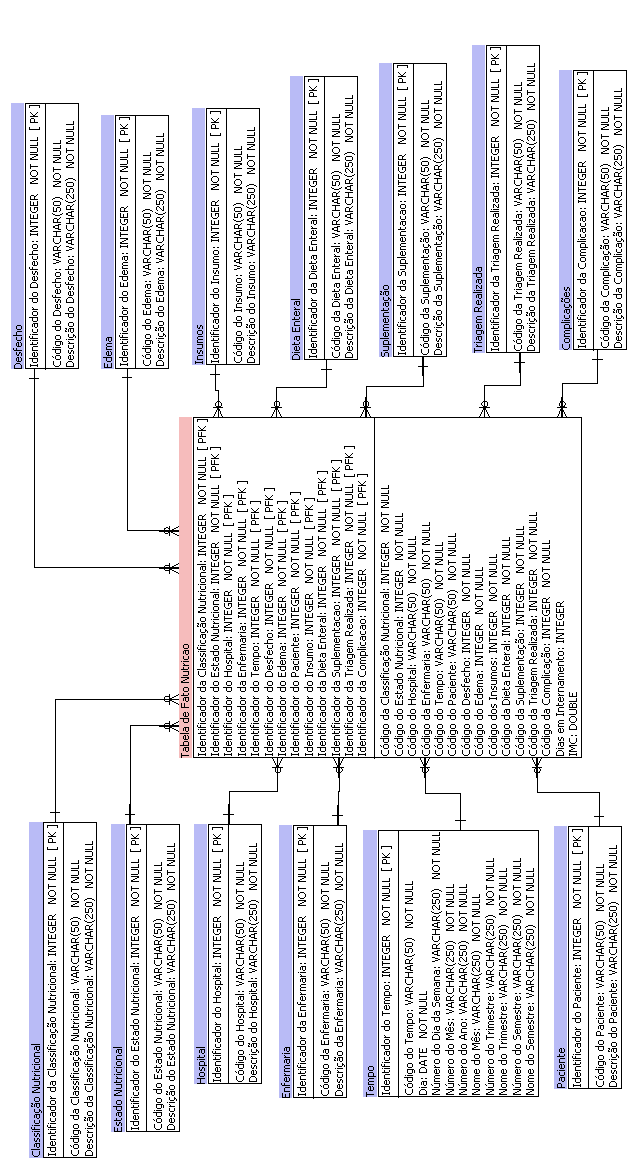
\includegraphics[scale=0.59]{Imagens/figura - modelagem multidimensional datamart.png}
	\end{center}
	\legend{Fonte: Autor.}
\end{figure}

O projeto multidimensional e o projeto do cubo ROLAP foram construídos com a ferramenta SQL \textit{Power Architect}, que além da concepção, auxilia na geração e execução do \textit{script} de criação tanto do \textit{Data Warehouse}, quanto do \textit{Data Mart}, implementados na sintaxe do PostgreSQL. Além de ser um SGBD robusto e gratuito, o PostgreSQL também é o sistema de gerenciamento de banco de dados utilizado pelo HU. 

\subsection{Processo de Extração, Transformação e Carga}
Com o modelo dimensional construído, foi dada sequência à próxima etapa do projeto, o desenvolvimento do processo de extração, transformação e carga. Para a fase de ETL foi utilizado o \textit{Pentaho Data Integration} (PDI), ferramenta da Pentaho utilizada para sistematizar o processo de tratamento e limpeza dos dados oriundos das fontes de dados e inserção nos armazéns de dados e nos \textit{Data Marts}.

A partir dos arquivos disponibilizados pela Unidade de Nutrição, em formato de planilha eletrônica do \textit{Microsoft Office}, foram corrigidos, padronizados e tratados todos os desvios e inconsistências encontradas. Sequencialmente foi iniciada a carga dos dados no DW, concluindo a persistência dos dados consolidados. Foram desenvolvidos um \textit{script} ETL para cada dimensão e um \textit{script} para a tabela de fato, resultando em 14 \textit{scripts} ETL. A seguir, na \autoref{fig_etldimensaohospital} está o processo de transformação utilizado para a carga das informações do hospital. 

\begin{figure}[htb]
	\caption{\label{fig_etldimensaohospital}Processo ETL para a Dimensão Hospital.}
	\begin{center}
	    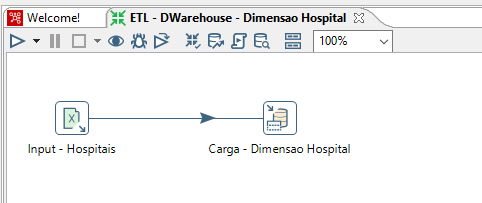
\includegraphics[scale=0.8]{Imagens/figura - etl dw hospital.png}
	\end{center}
	\legend{Fonte: Autor.}
\end{figure}

Na \autoref{fig_etldimensaoenfermaria} os dados relacionados as enfermarias do Hospital Universitário foram obtidos do banco de dados do Aplicativo de Gestão para Hospitais Universitários (AGHU). 
\begin{figure}[htb]
	\caption{\label{fig_etldimensaoenfermaria}Processo ETL para a Dimensão Enfermaria.}
	\begin{center}
	    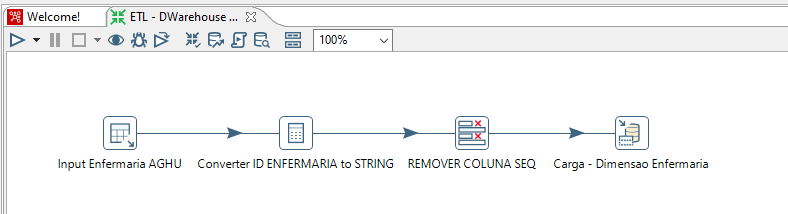
\includegraphics[scale=0.7]{Imagens/figura - etl dw enfermaria.png}
	\end{center}
	\legend{Fonte: Autor.}
\end{figure}

Na \autoref{fig_etldimensaotriagem} está o processo de transformação utilizado para a carga das informações de triagens nutricionais.

\begin{figure}[htb]
	\caption{\label{fig_etldimensaotriagem}Processo ETL para a Dimensão Triagem Realizada.}
	\begin{center}
	    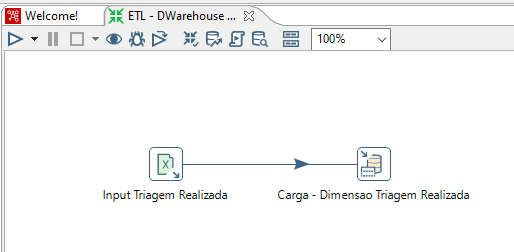
\includegraphics[scale=0.7]{Imagens/figura - etl dw triagem.png}
	\end{center}
	\legend{Fonte: Autor.}
\end{figure}

Na \autoref{fig_etldimensaotempo} está o processo de transformação utilizado para a carga das informações da Dimensão Tempo.

\begin{figure}[htb]
	\caption{\label{fig_etldimensaotempo}Processo ETL para a Dimensão Tempo.}
	\begin{center}
	    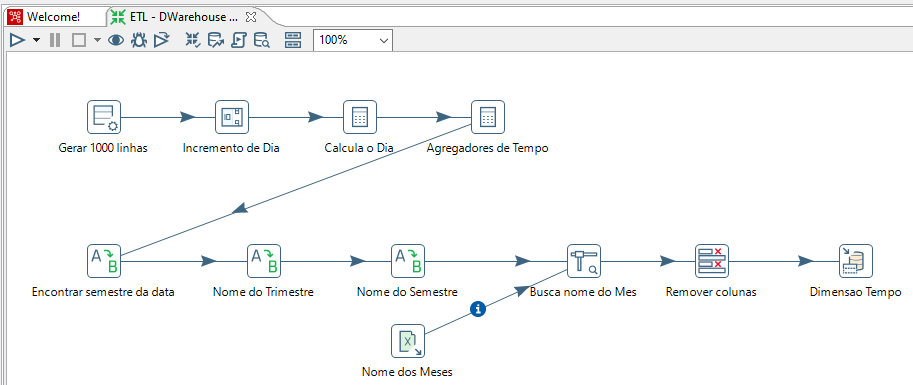
\includegraphics[scale=0.6]{Imagens/figura - etl dw tempo.png}
	\end{center}
	\legend{Fonte: Autor.}
\end{figure}

\newpage
Na \autoref{fig_etldimensaopaciente} está o processo de transformação utilizado para a carga das informações da Dimensão Paciente.

\begin{figure}[htb]
	\caption{\label{fig_etldimensaopaciente}Processo ETL para a Dimensão Paciente.}
	\begin{center}
	    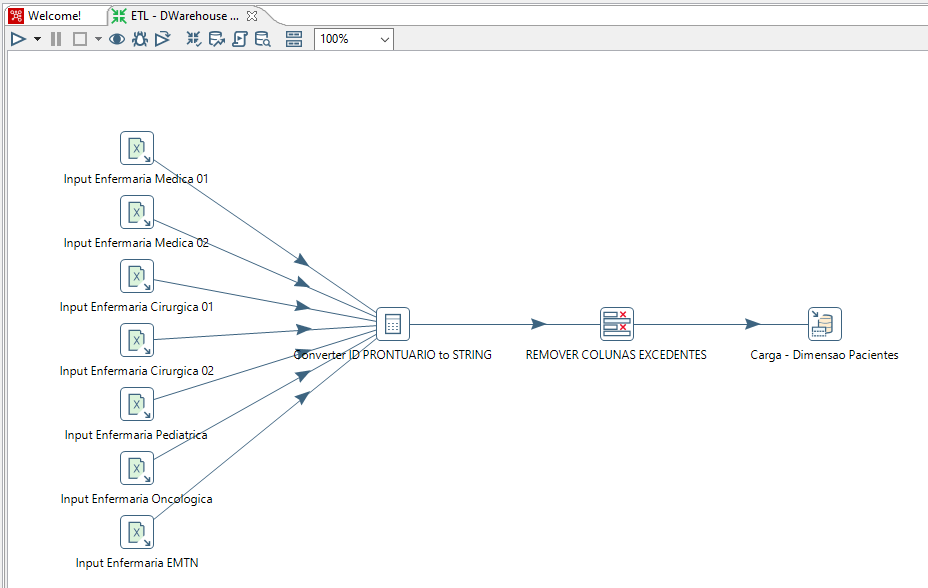
\includegraphics[scale=0.6]{Imagens/figura - etl dw paciente.png}
	\end{center}
	\legend{Fonte: Autor.}
\end{figure}

Na \autoref{fig_etldimensaosuplementacao} está o processo de transformação utilizado para a carga das informações de suplementação.

\begin{figure}[htb]
	\caption{\label{fig_etldimensaosuplementacao}Processo ETL para a Dimensão Suplementação.}
	\begin{center}
	    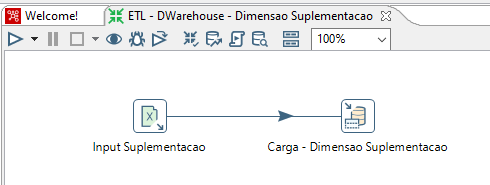
\includegraphics[scale=0.8]{Imagens/figura - etl dw suplementacao.png}
	\end{center}
	\legend{Fonte: Autor.}
\end{figure}

\newpage
A seguir, na \autoref{fig_etldimensaoinsumo} está o processo de transformação utilizado para a carga das informações da Dimensão Insumo.

\begin{figure}[htb]
	\caption{\label{fig_etldimensaoinsumo}Processo ETL para a Dimensão Insumos.}
	\begin{center}
	    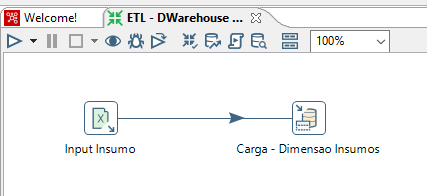
\includegraphics[scale=0.7]{Imagens/figura - etl dw insumos.png}
	\end{center}
	\legend{Fonte: Autor.}
\end{figure}

Na \autoref{fig_etldimensaoestado} está o processo de transformação utilizado para a carga das informações de estado nutricional.

\begin{figure}[htb]
	\caption{\label{fig_etldimensaoestado}Processo ETL para a Dimensão Estado Nutricional.}
	\begin{center}
	    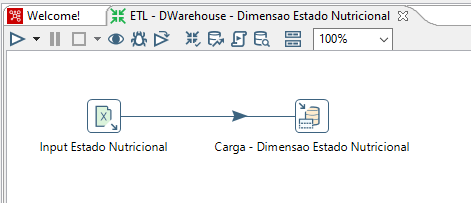
\includegraphics[scale=0.7]{Imagens/figura - etl dw estadonutricional.png}
	\end{center}
	\legend{Fonte: Autor.}
\end{figure}

A seguir, na \autoref{fig_etldimensaoedema} está o processo de transformação utilizado para a carga das informações da Dimensão Edema.
\begin{figure}[htb]
	\caption{\label{fig_etldimensaoedema}Processo ETL para a Dimensão Edema.}
	\begin{center}
	    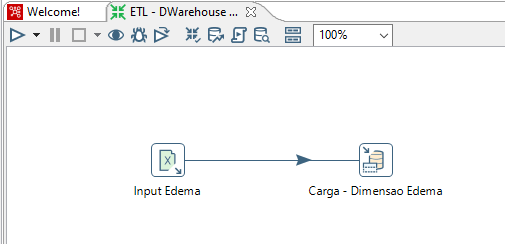
\includegraphics[scale=0.7]{Imagens/figura - etl dw edema.png}
	\end{center}
	\legend{Fonte: Autor.}
\end{figure}

Na \autoref{fig_etldimensaodesfecho} está o processo de transformação utilizado para a carga das informações da Dimensão Desfecho.
\begin{figure}[htb]
	\caption{\label{fig_etldimensaodesfecho}Processo ETL para a Dimensão Desfecho.}
	\begin{center}
	    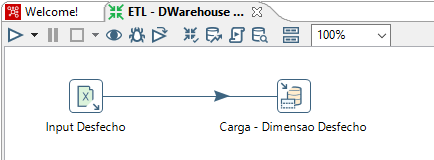
\includegraphics[scale=0.75]{Imagens/figura - etl dw desfecho.png}
	\end{center}
	\legend{Fonte: Autor.}
\end{figure}

Na \autoref{fig_etldimensaoentetal} está o processo de transformação utilizado para a carga das informações de dieta enteral.
\begin{figure}[htb]
	\caption{\label{fig_etldimensaoentetal}Processo ETL para a Dimensão Dieta Enteral.}
	\begin{center}
	    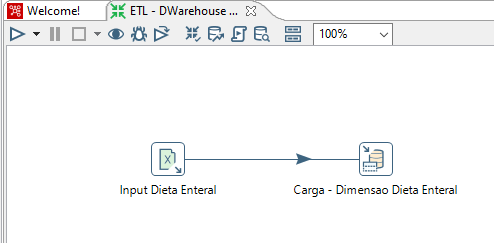
\includegraphics[scale=0.75]{Imagens/figura - etl dw dietaenteral.png}
	\end{center}
	\legend{Fonte: Autor.}
\end{figure}

Na \autoref{fig_etldimensaocomplicacoes} está o processo de transformação utilizado para a carga das informações da Dimensão Complicações.
\begin{figure}[htb]
	\caption{\label{fig_etldimensaocomplicacoes}Processo ETL para a Dimensão Complicações.}
	\begin{center}
	    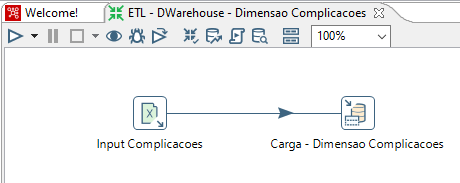
\includegraphics[scale=0.75]{Imagens/figura - etl dw complicacoes.png}
	\end{center}
	\legend{Fonte: Autor.}
\end{figure}

Na \autoref{fig_etldimensaoclassificacao} está o processo de transformação utilizado para a carga das informações de classificação nutricional.
\begin{figure}[htb]
	\caption{\label{fig_etldimensaoclassificacao}Processo ETL para a Dimensão Classificação Nutricional.}
	\begin{center}
	    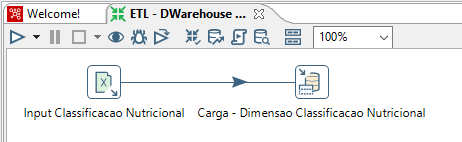
\includegraphics[scale=0.9]{Imagens/figura - etl dw classificacao.png}
	\end{center}
	\legend{Fonte: Autor.}
\end{figure}

A \autoref{fig_etltabelafato} mostra o processo de transformação e carga para a Tabela de Fato do \textit{Data Warehouse}. 
\begin{figure}[htb]
	\caption{\label{fig_etltabelafato}Processo ETL para a Tabela de Fato do \textit{Data Warehouse}.}
	\begin{center}
	    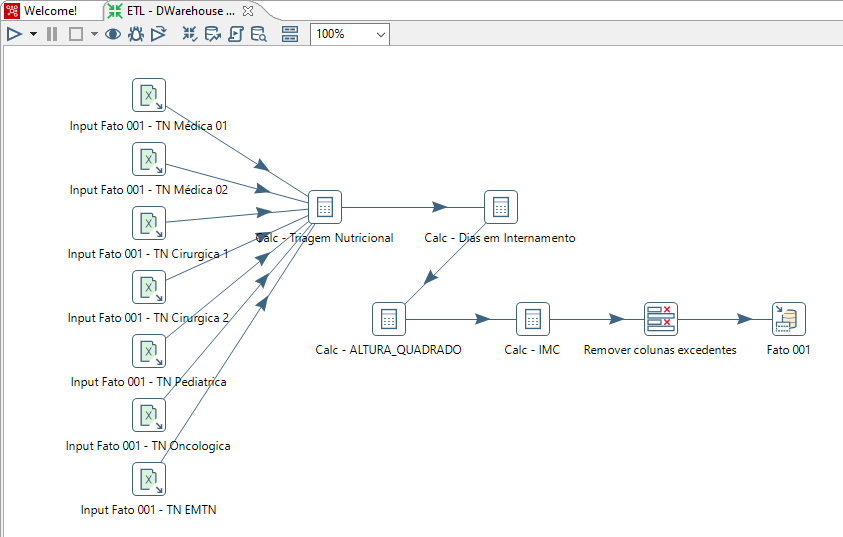
\includegraphics[scale=0.75]{Imagens/figura - etl dw fato.png}
	\end{center}
	\legend{Fonte: Autor.}
\end{figure}

\newpage
Na \autoref{fig_etlcargafatodatamart} está representado o processo de transformação e carga para a tabela fato do \textit{Datamart}. 
\begin{figure}[htb]
	\caption{\label{fig_etlcargafatodatamart}Processo ETL para a Tabela de Fato do \textit{Datamart}.}
	\begin{center}
	    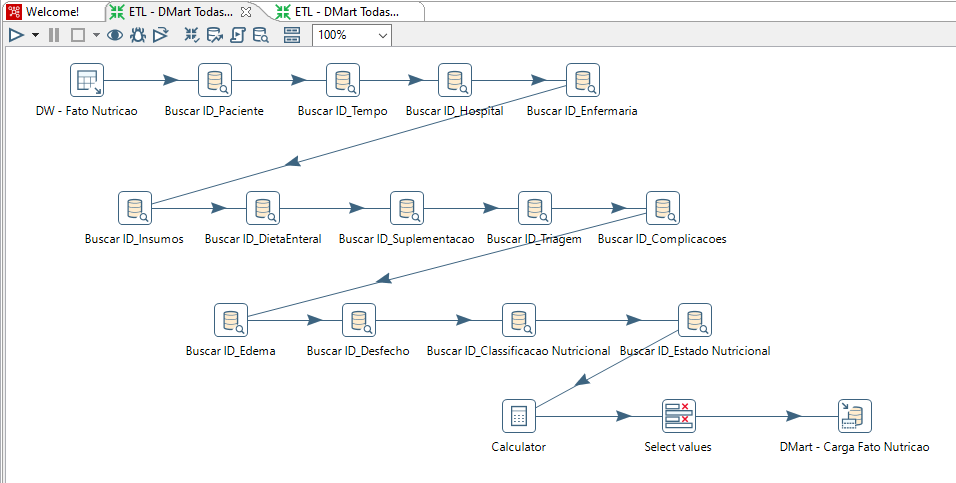
\includegraphics[scale=0.57]{Imagens/figura - etl dm fato.png}
	\end{center}
	\legend{Fonte: Autor.}
\end{figure}

Já na \autoref{fig_etlcargadimensoesdatamart} está representado o processo para as dimensões do \textit{Datamart}.
\begin{figure}[htb]
	\caption{\label{fig_etlcargadimensoesdatamart}Processo ETL para as Dimensões do \textit{Datamart}.}
	\begin{center}
	    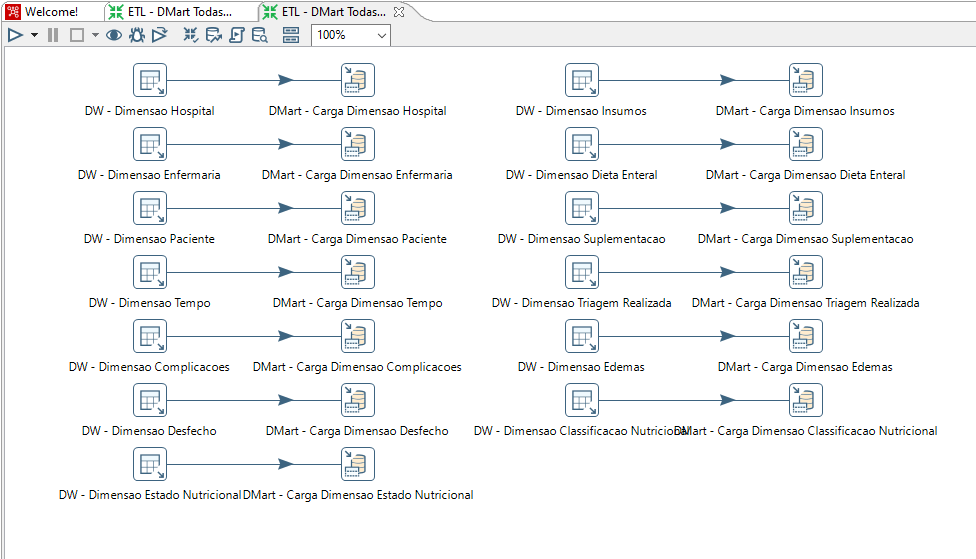
\includegraphics[scale=0.56]{Imagens/figura - etl dm dimensoes.png}
	\end{center}
	\legend{Fonte: Autor.}
\end{figure}
\clearpage

\subsection{Mapeamento e Consultas OLAP}
Com o processo de carga completo, o próximo passo da sequência é a configuração e criação do cubo lógico de dados com as propriedades das medidas e dimensões, como funções de agregação, formatação, funções matemáticas e nome para exibição. A ferramenta utilizada foi o \textit{Pentaho Schema Workbench} que também é fornecida no pacote \textit{Pentaho Community} e usa o mecanismo Modrian para se comunicar com os esquemas ROLAP e processar as solicitações de consultas multidimensionais, também conhecidas em inglês como \textit{Multidimensional Express} (MDX). A \autoref{fig_pentahoshemaworkbench} apresenta o cubo lógico "DMNutricao", onde estão definidas as medidas: "ClassificacaoDeRisco", "EstadoNutricional", "Desfecho", "Edema", "Insumo", "DietaEnteral", "UsoDeSuplemento", "TriagemRealizada", "Complicacoes" e "DiasInternamento" que são utilizados para geração dos \textit{dashboards}, utilizando todas as Dimensões de acordo com modelo relacional da \autoref{fig_modelagemdatamart}.

\begin{figure}[htb]
	\caption{\label{fig_pentahoshemaworkbench}Modelagem do cubo lógico de dados.}
	\begin{center}
	    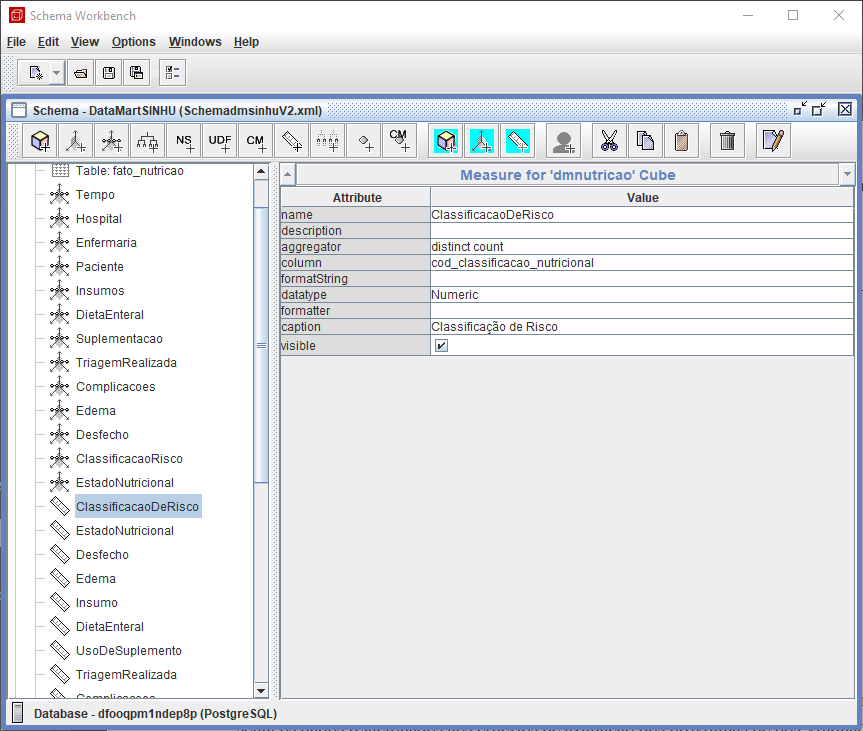
\includegraphics[scale=0.65]{Imagens/figura - schema workbench.png}
	\end{center}
	\legend{Fonte: Autor.}
\end{figure}

\newpage
As consultas MDX que são a base dos relatórios e gráficos, podem ser montadas e testadas no ambiente de \textit{query} do próprio \textit{Schema Workcbench}, a \autoref{fig_shemaworkbenchconsulta} mostra a consulta MDX realizada para o relatório de quantidade de triagens realizadas por mês para cada enfermaria do hospital. Na área em amarelo é escrita a \textit{query} de consulta e na área em vermelho é mostrada a resposta da consulta multidimensional.
\begin{figure}[htb]
	\caption{\label{fig_shemaworkbenchconsulta}Exemplo de consulta MDX no Schema Workbench.}
	\begin{center}
	    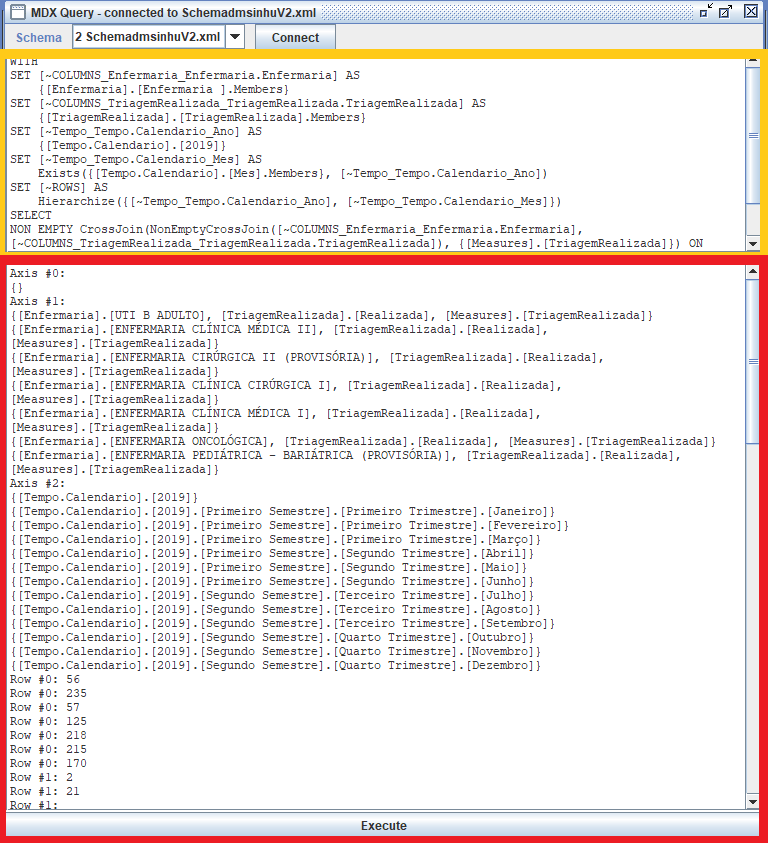
\includegraphics[scale=0.7]{Imagens/figura - workbenchconsulta.png}
	\end{center}
	\legend{Fonte: Autor.}
\end{figure}

\newpage
\subsection{Ambiente de Relatórios}
Com o ambiente pronto e as consultas necessárias montadas, é possível seguir à etapa de geração dos relatórios e \textit{dashboards} no \textit{Pentaho Business Analytics Platform}. A plataforma de \textit{Business Analytics} conta com o editor padrão de relatórios \textit{JPivot View}, mas também é permitida a instalação de outras bibliotecas, que podem ser integradas por meio do \textit{Marketplace} da Pentaho ou instaladas manualmente quando de fontes externas. O \textit{JPivot} em sua versão disponibilizada de forma padrão no \textit{Pentaho Server} recebeu sua última atualização em 17 de março de 2008, indicando certa descontinuidade por parte da comunidade e por este motivo para este trabalho foi instalada a biblioteca \textit{Saiku Analytics}, um cliente web disponível em forma de \textit{plugin} no \textit{Marketplace}, como mostra a \autoref{fig_pluginsaiku}. 
\begin{figure}[htb]
	\caption{\label{fig_pluginsaiku}\textit{Plugin Saiku Analytics} no \textit{Pentaho Marketplace}.}
	\begin{center}
	    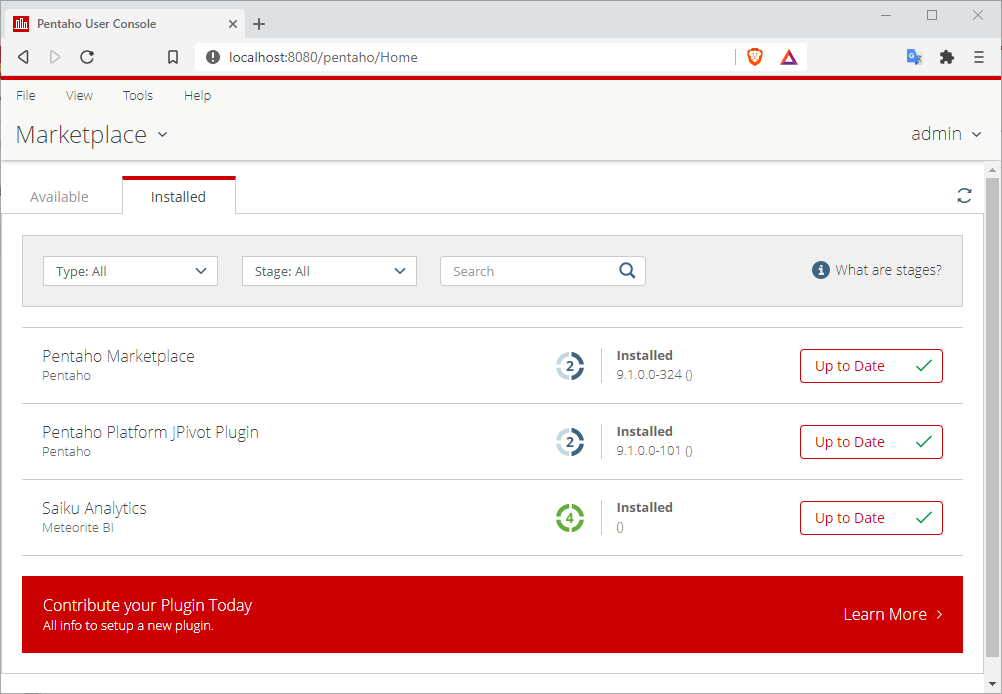
\includegraphics[scale=0.6]{Imagens/figura - pluginsaiku.png}
	\end{center}
	\legend{Fonte: Autor.}
\end{figure}

\newpage
O ambiente para montagem dos relatórios pode ser conferido na \autoref{fig_saikuanalytics}.
Ele também utiliza o motor Mondrian para as consultas aos cubos ROLAP. 

\begin{figure}[htb]
	\caption{\label{fig_saikuanalytics}Ambiente de relatórios do \textit{Saiku Analytics}.}
	\begin{center}
	    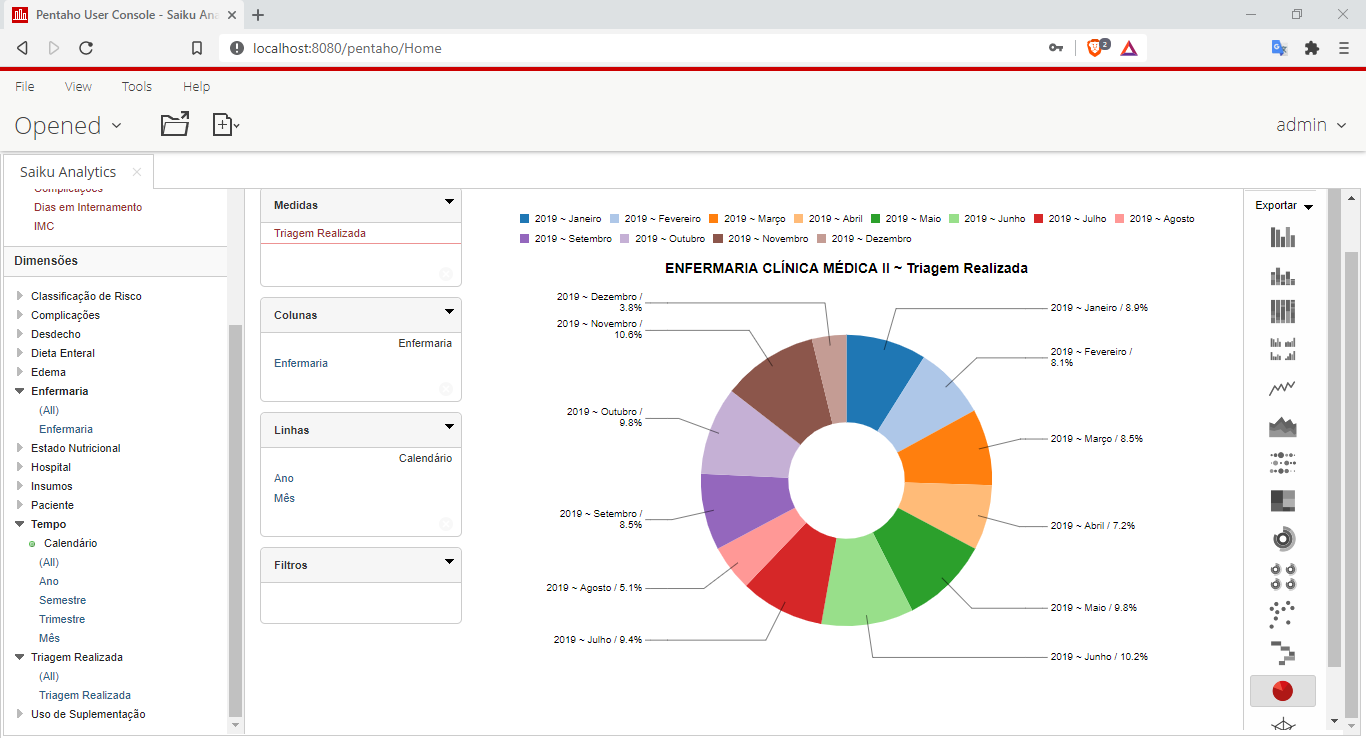
\includegraphics[scale=0.45]{Imagens/figura - saikudashboard.png}
	\end{center}
	\legend{Fonte: Autor.}
\end{figure}

Também permite que o usuário final elabore as próprias consultas com vários gráficos disponíveis e função arrastar e soltar (\textit{drag in drop}) tornando a experiência mais intuitiva, dispensando conhecimento prévio em SQL ou MDX. 

\section{Resultados e Discursões}

A plataforma de integração e análise de dados da Pentaho permite que as organizações acessem, preparem e analisem todos os dados de qualquer fonte, em qualquer ambiente \cite{pentahosite}. E o \textit{Saiku Analytics} permite realizar análises complexas e poderosas usando uma interface fácil, arrastando e soltando as medidas e dimensões por meio do navegador criando relatórios detalhados e ótimas visualizações gráficas \cite{meteoribisite}. A seguir, estão  os resultados obtidos conforme as demandas solicitadas pela Unidade de Nutrição Clínica do HU-UFS.

\subsection{Relatórios e \textit{Dashboards} Obtidos}
Com o ambiente de relatórios pronto e as consultas carregadas utilizando o \textit{Saiku Analytics} foi possível gerar os relatórios com as informações solicitadas pela Unidade de Nutrição Clínica do Hospital Universitário. A \autoref{dashboard_TotalTriagensRealizadasHospitalAnoTabela}, mostra a quantidade de triagens nutricionais realizadas no ano de 2019.

\begin{figure}[htb]
	\caption{\label{dashboard_TotalTriagensRealizadasHospitalAnoTabela}Quantidade de Triagens Nutricionais Realizadas.}
	\begin{center}
	    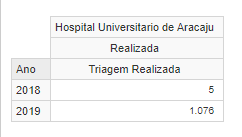
\includegraphics[scale=1]{Imagens/1.1.TotalTriagensRealizadasHospitalAnoTabela.png}
	\end{center}
	\legend{Fonte: Autor.}
\end{figure}

A \autoref{dashboard_TotalTriagensRealizadasHospitalMesTabela}, mostra o relatório com a quantidade de triagens nutricionais realizadas por mês durante o ano de 2019. 

\begin{figure}[htb]
	\caption{\label{dashboard_TotalTriagensRealizadasHospitalMesTabela}Quantidade de Triagens Nutricionais Realizadas ao mês.}
	\begin{center}
	    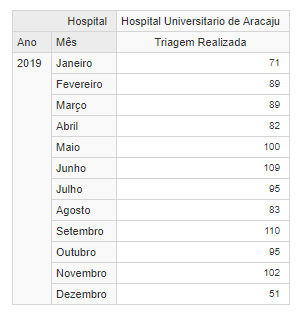
\includegraphics[scale=1]{Imagens/1.2.TotalTriagensRealizadasHospitalMesTabela.png}
	\end{center}
	\legend{Fonte: Autor.}
\end{figure}

A \autoref{dashboard_TotalTriagensRealizadasEnfermariaAnoBarras}, mostra o gráfico de barras sobre a quantidade de triagens nutricionais realizadas por enfermaria no ano de 2019.

\newpage
\begin{figure}[htb]
	\caption{\label{dashboard_TotalTriagensRealizadasEnfermariaAnoBarras}Quantidade de Triagens Nutricionais Realizadas por enfermaria.}
	\begin{center}
	    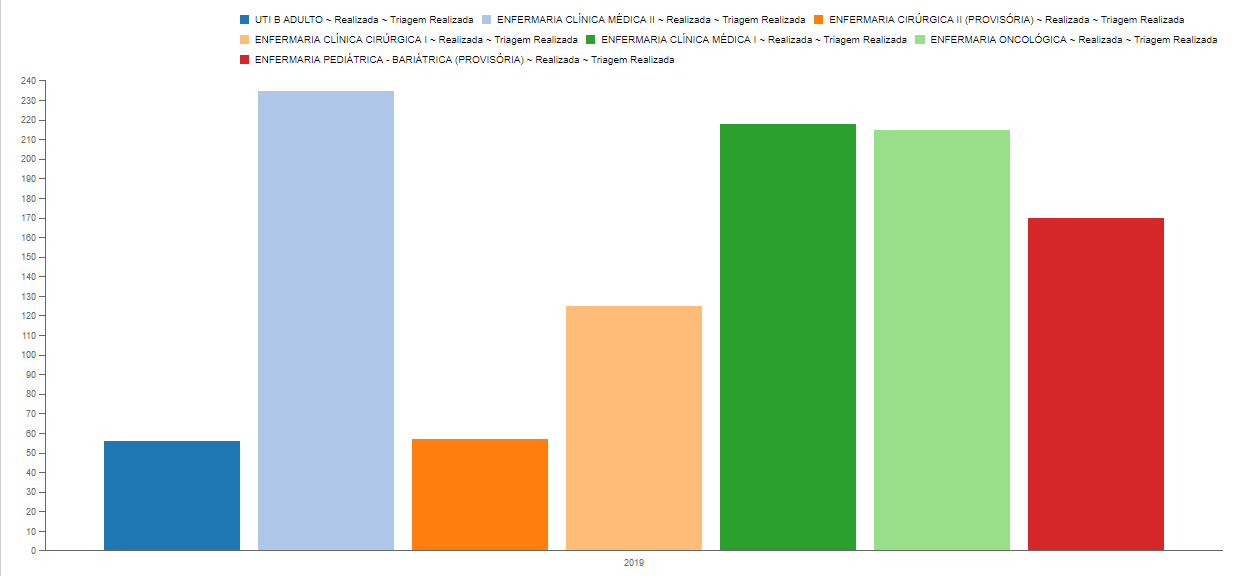
\includegraphics[scale=0.4]{Imagens/1.3.TotalTriagensRealizadasEnfermariaAnoBarras.png}
	\end{center}
	\legend{Fonte: Autor.}
\end{figure}

A \autoref{dashboard_TotalTriagensRealizadasEnfermariaMesLinhas}, contém um gráfico de linhas demonstrando a tendência de triagens nutricionais realizadas por enfermaria no ano de 2019.

\begin{figure}[htb]
	\caption{\label{dashboard_TotalTriagensRealizadasEnfermariaMesLinhas}Tendência de Triagens Nutricionais Realizadas por enfermaria.}
	\begin{center}
	    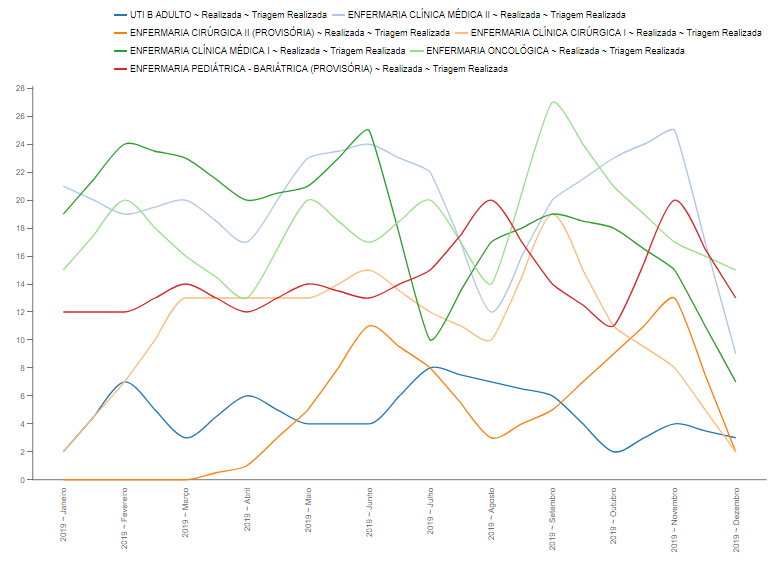
\includegraphics[scale=0.63]{Imagens/1.4.TotalTriagensRealizadasEnfermariaMesLinhas.png}
	\end{center}
	\legend{Fonte: Autor.}
\end{figure}

\newpage
A \autoref{dashboard_PercentualClassificacaoRiscoHospitalAnoPizza}, mostra o gráfico de pizza do percentual de pacientes segundo classificação de risco no ano de 2019.

\begin{figure}[htb]
	\caption{\label{dashboard_PercentualClassificacaoRiscoHospitalAnoPizza}Percentual de Pacientes segundo Classificação de Risco.}
	\begin{center}
	    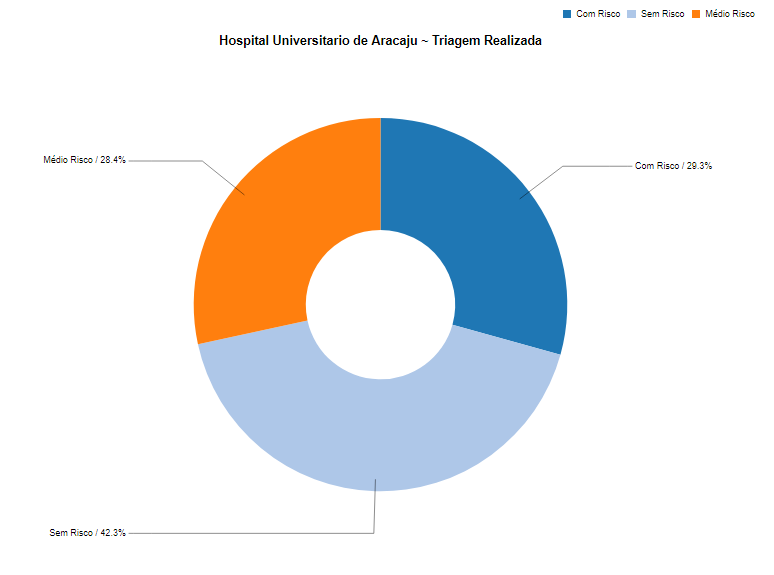
\includegraphics[scale=0.6]{Imagens/2.1.PercentualPacientesClassificacaoRiscoHospitalAnoPizza.png}
	\end{center}
	\legend{Fonte: Autor.}
\end{figure}

\clearpage
A \autoref{dashboard_PercentualPacientesClassificacaoRiscoHospitalMesPizza}, mostra o percentual de classificação de risco por triagem nutricional por mês durante o ano de 2019.

\begin{figure}[htb]
	\caption{\label{dashboard_PercentualPacientesClassificacaoRiscoHospitalMesPizza}Percentual de Pacientes segundo Classificação de Risco detalhado por mês.}
	\begin{center}
	    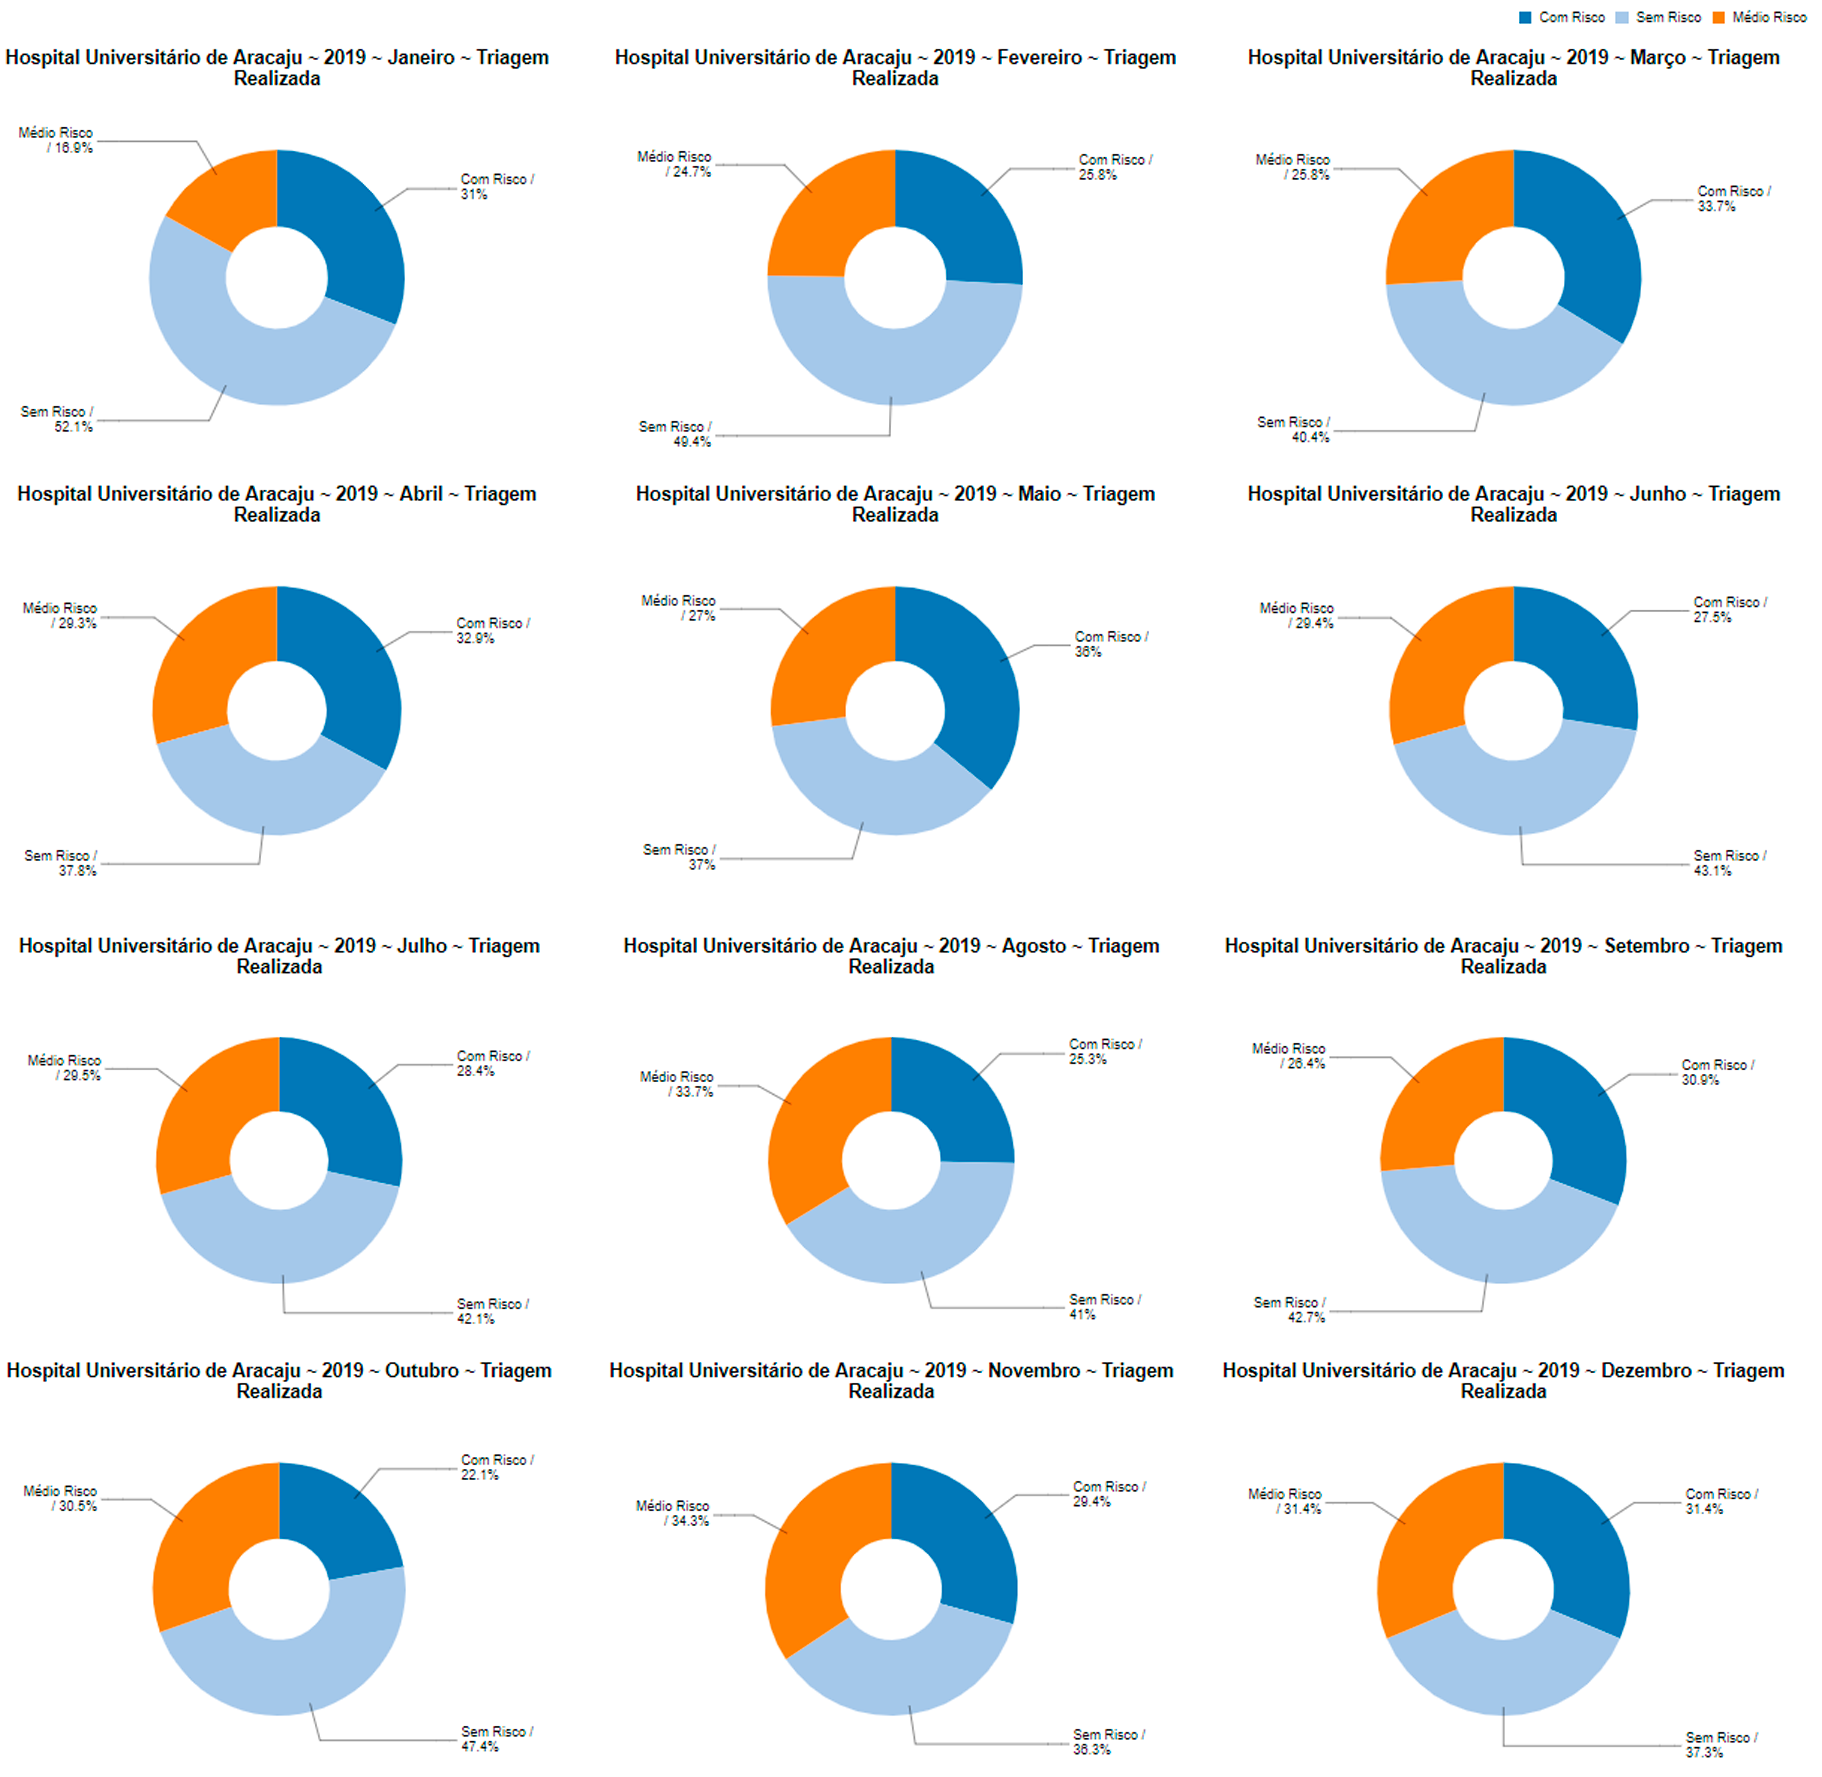
\includegraphics[scale=0.6]{Imagens/2.2.PercentualPacientesClassificacaoRiscoHospitalMesPizza.png}
	\end{center}
	\legend{Fonte: Autor.}
\end{figure}

\clearpage
A \autoref{dashboard_PercentualPacientesClassificacaoRiscoEnfermariaAnoPizza}, mostra o percentual de classificação risco por triagem nutricional no ano de 2019.

\begin{figure}[htb]
	\caption{\label{dashboard_PercentualPacientesClassificacaoRiscoEnfermariaAnoPizza}Percentual de Pacientes segundo Classificação de Risco por enfermaria.}
	\begin{center}
	    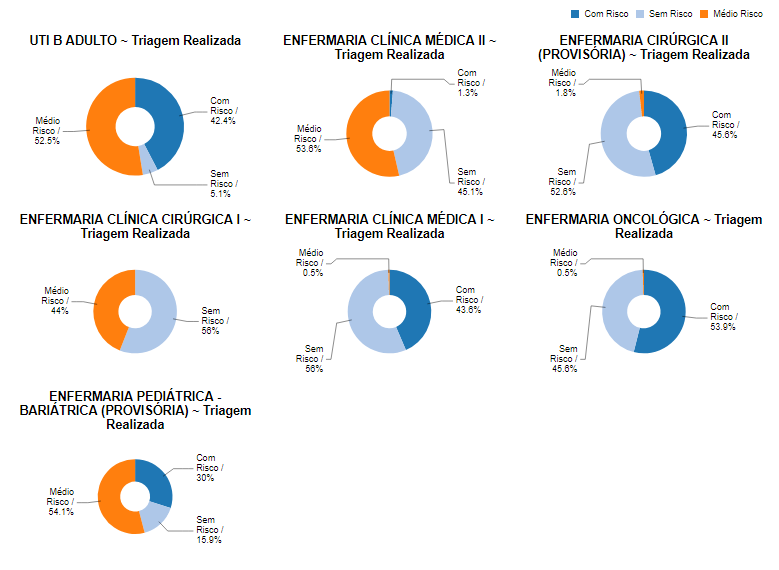
\includegraphics[scale=0.6]{Imagens/2.3.PercentualPacientesClassificacaoRiscoEnfermariaAnoPizza.png}
	\end{center}
	\legend{Fonte: Autor.}
\end{figure}

\clearpage
A \autoref{dashboard_PercentualPacientesClassificacaoRiscoEnfermariaMesLinha}, mostra a tendência de pacientes segundo classificação risco por enfermaria por mês ao longo do ano de 2019. O filtro detalha as informações de tendência da enfermaria Clínica Médica II.

\begin{figure}[htb]
	\caption{\label{dashboard_PercentualPacientesClassificacaoRiscoEnfermariaMesLinha}Tendência de Pacientes segundo Classificação de Risco por enfermaria detalhado por mês.}
	\begin{center}
	    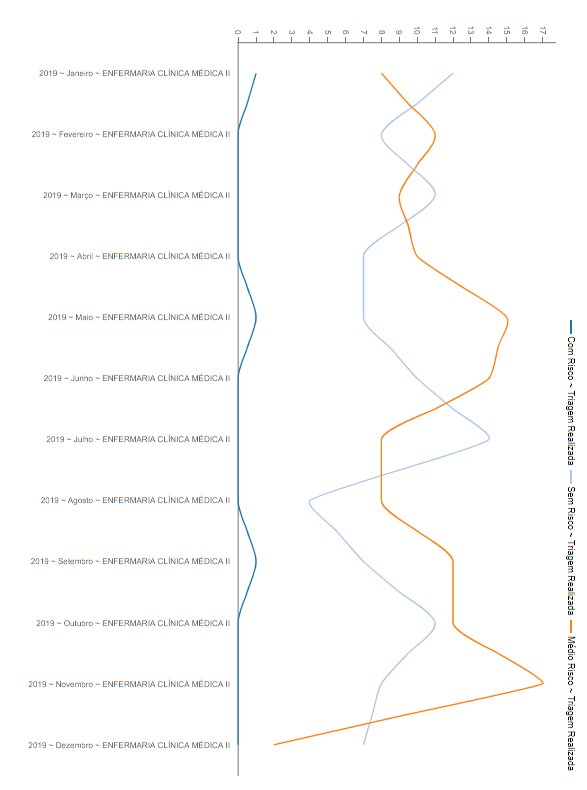
\includegraphics[scale=0.9]{Imagens/2.4.PercentualPacientesClassificacaoRiscoEnfermariaMesLinha.png}
	\end{center}
	\legend{Fonte: Autor.}
\end{figure}

\newpage
A \autoref{dashboard_PercentualPacienteEstadoNutricionalHospitalAnoPizza}, mostra o percentual de pacientes segundo estado nutricional no ano de 2019.

\begin{figure}[htb]
	\caption{\label{dashboard_PercentualPacienteEstadoNutricionalHospitalAnoPizza}Percentual de Pacientes segundo Estado Nutricional.}
	\begin{center}
	    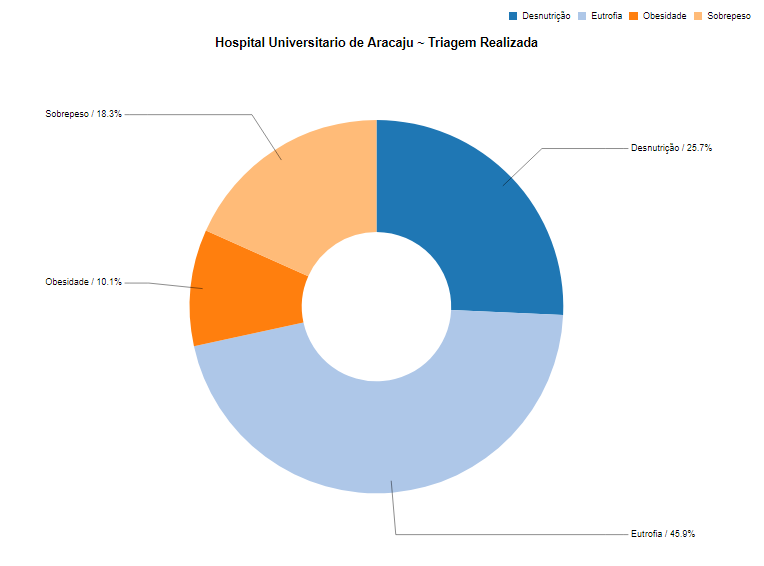
\includegraphics[scale=0.6]{Imagens/3.1.PercentualPacienteEstadoNutricionalHospitalAnoPizza.png}
	\end{center}
	\legend{Fonte: Autor.}
\end{figure}

\newpage
A \autoref{dashboard_PercentualPacienteEstadoNutricionalHospitalMesLinha}, mostra o percentual de pacientes segundo estado nutricional por mês.

\begin{figure}[htb]
	\caption{\label{dashboard_PercentualPacienteEstadoNutricionalHospitalMesLinha}Percentual de Pacientes segundo Estado Nutricional detalhado por mês.}
	\begin{center}
	    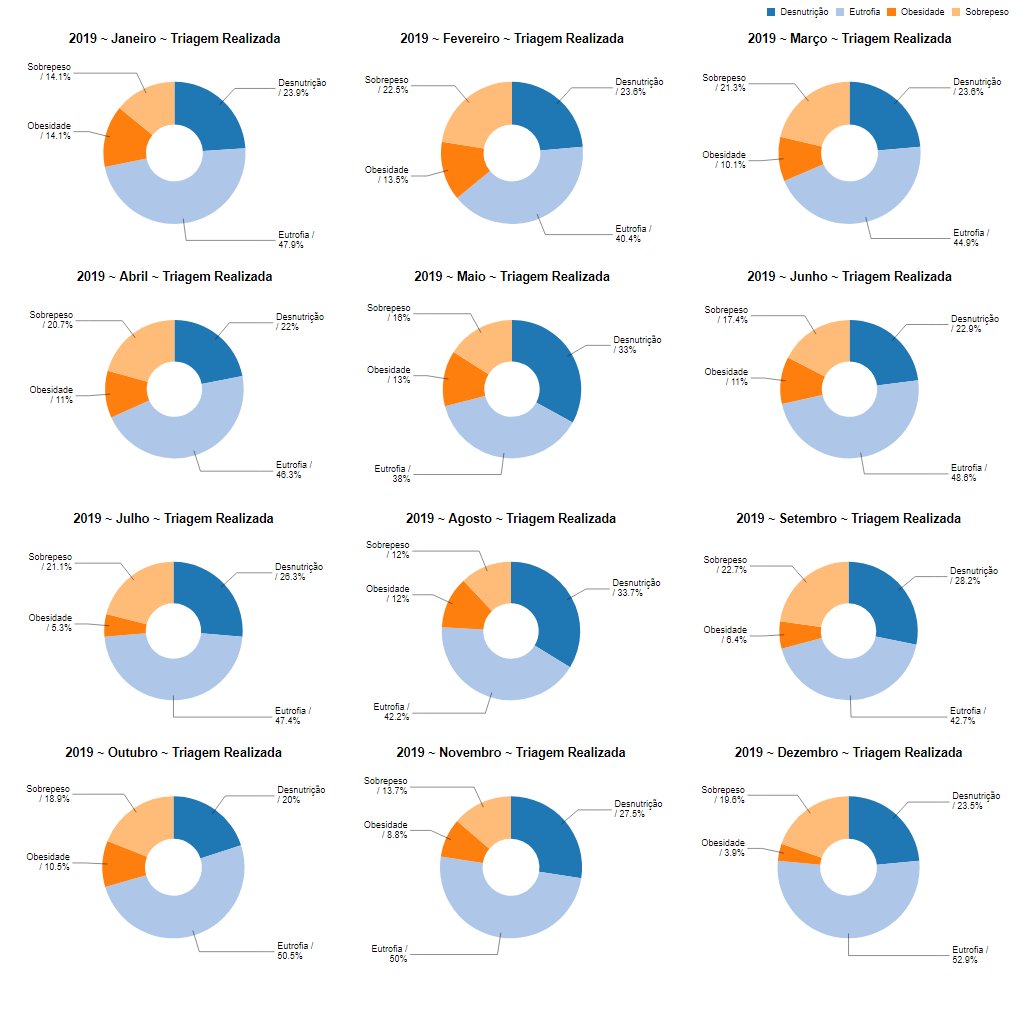
\includegraphics[scale=0.6]{Imagens/3.2.PercentualPacienteEstadoNutricionalHospitalMesLinha.png}
	\end{center}
	\legend{Fonte: Autor.}
\end{figure}

\newpage
A \autoref{dashboard_PercentualPacienteEstadoNutricionalEnfermariaAnoPizza}, mostra o percentual de pacientes segundo estado nutricional por enfermaria no ano de 2019.

\begin{figure}[htb]
	\caption{\label{dashboard_PercentualPacienteEstadoNutricionalEnfermariaAnoPizza}Percentual de Pacientes segundo Estado Nutricional por enfermaria.}
	\begin{center}
	    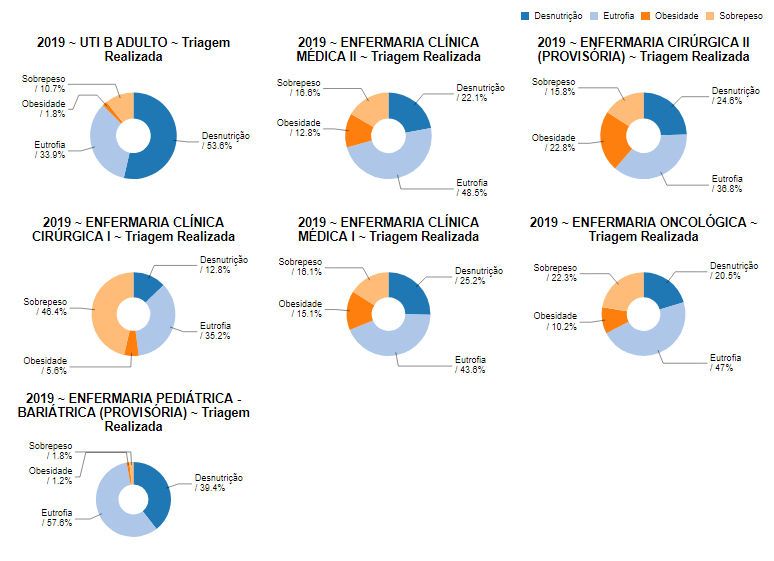
\includegraphics[scale=0.6]{Imagens/3.3.PercentualPacienteEstadoNutricionalEnfermariaAnoPizza.png}
	\end{center}
	\legend{Fonte: Autor.}
\end{figure}

\newpage
A \autoref{dashboard_PercentualPacienteEstadoNutricionalEnfermariaMesPizza}, mostra a tendência de pacientes segundo estado nutricional por enfermaria por mês ao longo do ano de 2019. O filtro detalha as informações de tendência da enfermaria Clínica Médica II.

\begin{figure}[htb]
	\caption{\label{dashboard_PercentualPacienteEstadoNutricionalEnfermariaMesPizza}Tendência de Pacientes segundo Estado Nutricional por Enfermaria detalhado por mês.}
	\begin{center}
	    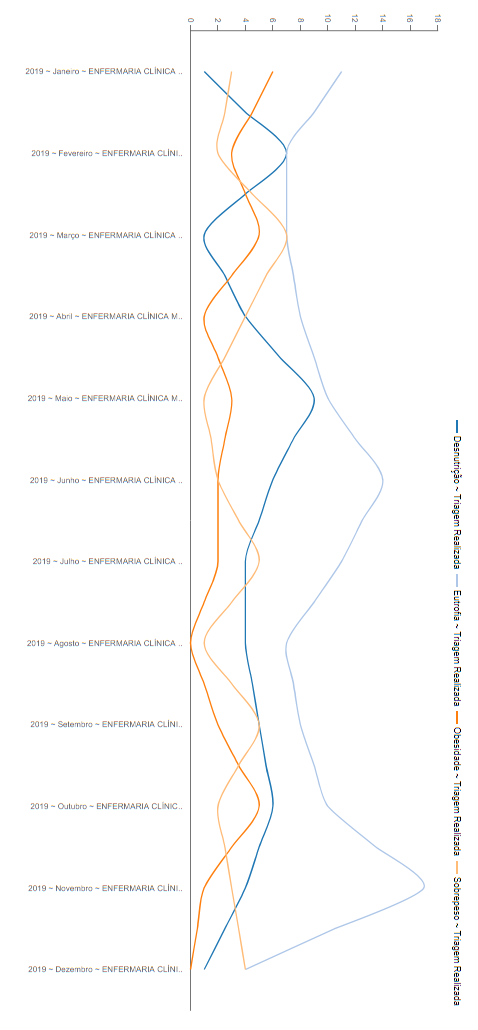
\includegraphics[scale=0.69]{Imagens/3.4.PercentualPacienteEstadoNutricionalEnfermariaMesPizza.png}
	\end{center}
	\legend{Fonte: Autor.}
\end{figure}

\newpage
A \autoref{dashboard_TotalUsoSuplementoHospitalAnoBarra}, mostra a quantidade de pacientes em uso de suplementação no ano de 2019.

\begin{figure}[htb]
	\caption{\label{dashboard_TotalUsoSuplementoHospitalAnoBarra}Quantidade de Pacientes em Uso de Suplemento.}
	\begin{center}
	    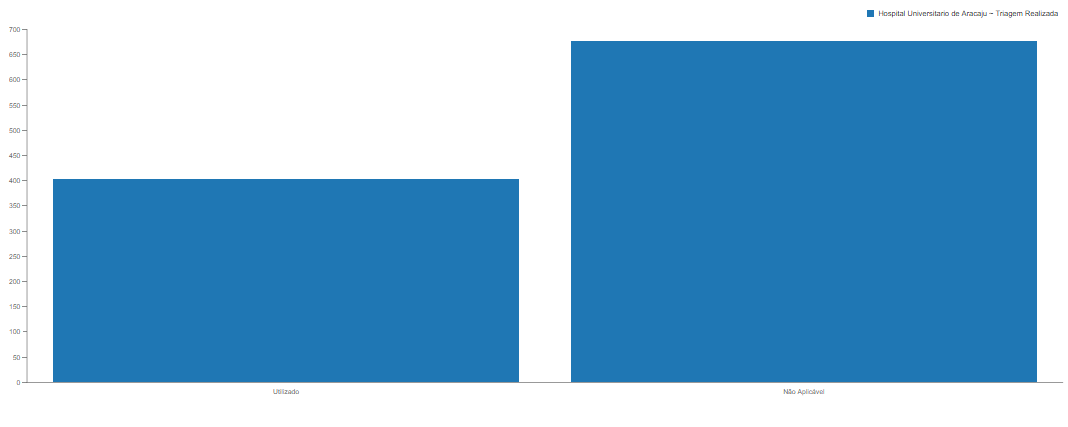
\includegraphics[scale=1]{Imagens/5.1.TotalUsoSuplementoHospitalAnoBarra.png}
	\end{center}
	\legend{Fonte: Autor.}
\end{figure}

A \autoref{dashboard_TotalUsoSuplementoEnfermariaAnoBarra}, mostra a quantidade de pacientes em uso de suplementação por enfermaria durante o ano de 2019.

\begin{figure}[htb]
	\caption{\label{dashboard_TotalUsoSuplementoEnfermariaAnoBarra}Quantidade de Pacientes em Uso de Suplemento por Enfermaria.}
	\begin{center}
	    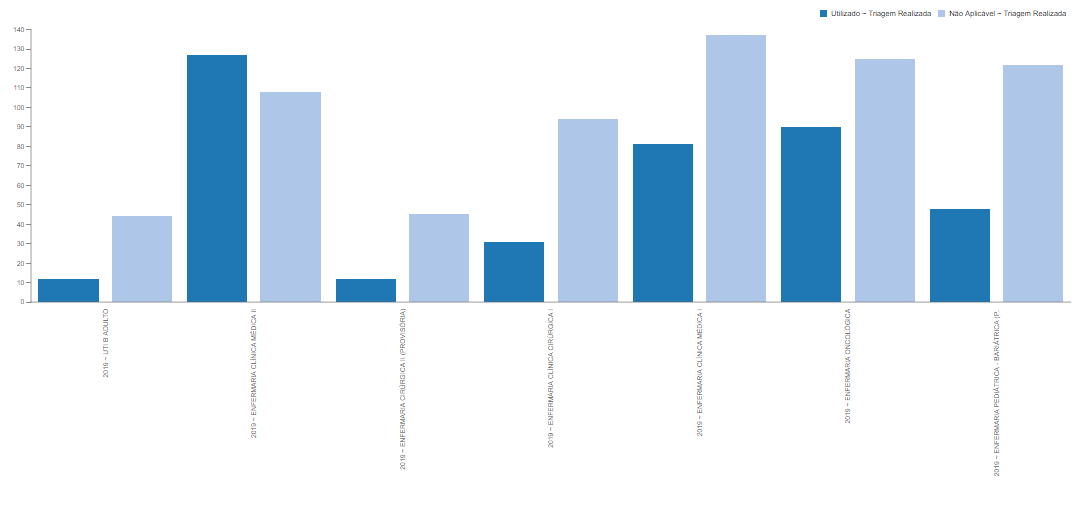
\includegraphics[scale=0.55]{Imagens/5.2.TotalUsoSuplementoEnfermariaAnoBarra.png}
	\end{center}
	\legend{Fonte: Autor.}
\end{figure}

\newpage
A \autoref{dashboard_PercentualPacienteUsoSuplementoHospitalAnoPizza}, mostra o percentual de pacientes segundo uso de suplementação no ano de 2019.

\begin{figure}[htb]
	\caption{\label{dashboard_PercentualPacienteUsoSuplementoHospitalAnoPizza}Percentual de Pacientes segundo Uso de Suplementação ao ano.}
	\begin{center}
	    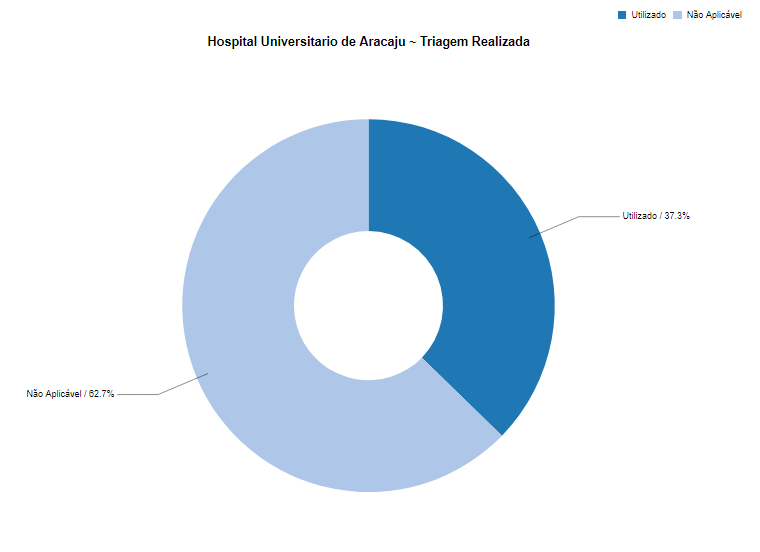
\includegraphics[scale=0.6]{Imagens/4.1.PercentualPacienteUsoSuplementoHospitalAnoPizza.png}
	\end{center}
	\legend{Fonte: Autor.}
\end{figure}

\newpage
A \autoref{dashboard_PercentualPacienteUsoSuplementoEnfermariaAnoPizza}, mostra o percentual de pacientes segundo uso de suplementação por enfermaria no ano de 2019.

\begin{figure}[htb]
	\caption{\label{dashboard_PercentualPacienteUsoSuplementoEnfermariaAnoPizza}Percentual de Pacientes segundo Uso de Suplementação por enfermaria.}
	\begin{center}
	    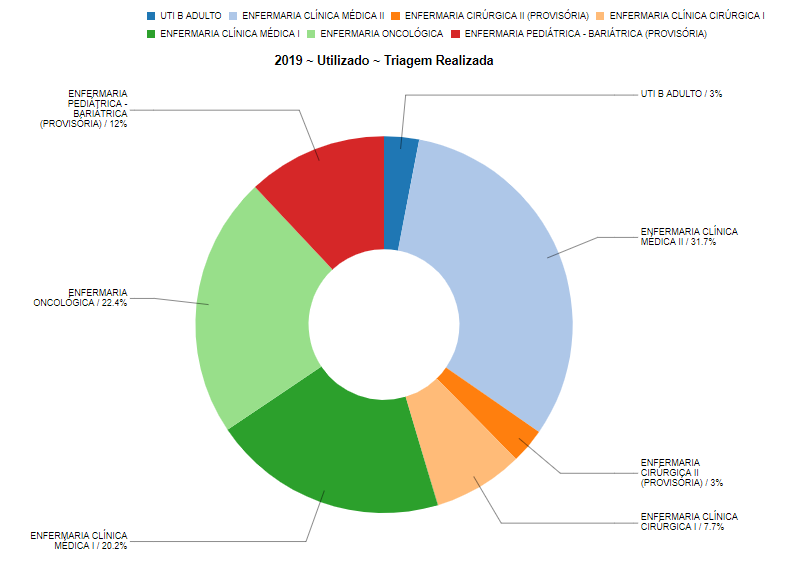
\includegraphics[scale=0.8]{Imagens/4.3.PercentualPacienteUsoSuplementoEnfermariaAnoPizza.png}
	\end{center}
	\legend{Fonte: Autor.}
\end{figure}

\newpage
A \autoref{dashboard_PercentualPacienteUsoSuplementoEnfermariaMesLinha}, mostra a tendência de pacientes segundo uso de suplementação por enfermaria durante o ano de 2019.  O filtro detalha as informações de tendência da enfermaria Clínica Médica II.

\begin{figure}[htb]
	\caption{\label{dashboard_PercentualPacienteUsoSuplementoEnfermariaMesLinha}Tendência de Pacientes segundo Uso de Suplementação por Enfermaria detalhado por mês.}
	\begin{center}
	    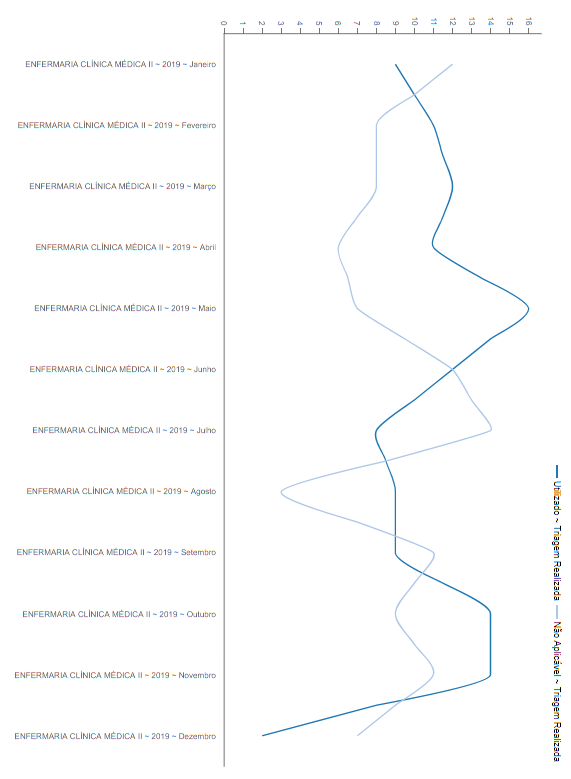
\includegraphics[scale=0.9]{Imagens/4.4.PercentualPacienteUsoSuplementoEnfermariaMesLinha.png}
	\end{center}
	\legend{Fonte: Autor.}
\end{figure}

\newpage
A \autoref{dashboard_TotalUsoSuplementoMediaDeDiasInternadoHospitalMesBarra}, mostra um comparativo entre os pacientes que utilizam suplementação com a média de dias em internamento, ao longo do ano de 2019.

\begin{figure}[htb]
	\caption{\label{dashboard_TotalUsoSuplementoMediaDeDiasInternadoHospitalMesBarra}Comparativo de pacientes que utilizam Suplementação com média de dias internado.}
	\begin{center}
	    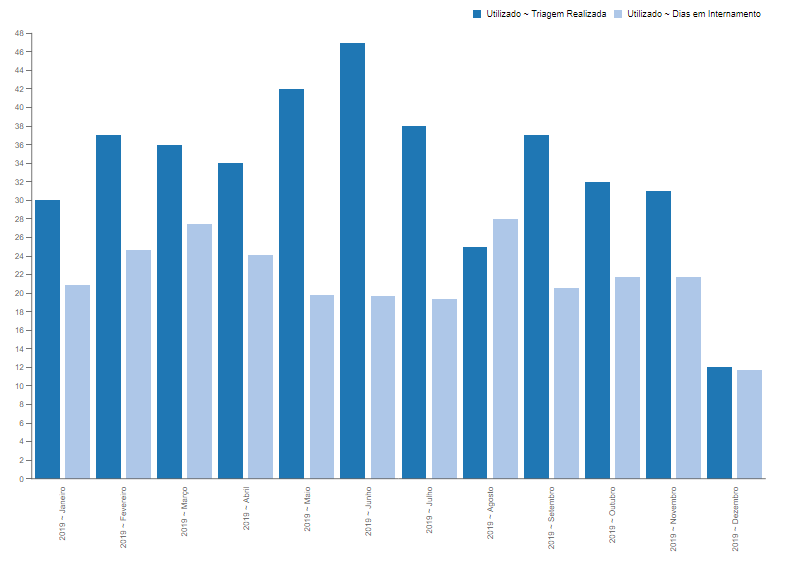
\includegraphics[scale=0.35]{Imagens/6.1.TotalUsoSuplementoMediaDeDiasInternadoHospitalMesBarra.png}
	\end{center}
	\legend{Fonte: Autor.}
\end{figure}

%\newpage
A \autoref{dashboard_TotalUsoSuplementoMediaDeDiasInternadoEnfermariaMesBarra}, mostra um comparativo entre os pacientes que utilizam suplementação com a média de dias em internamento por enfermaria durante o ano de 2019. O filtro detalha as informações de tendência da enfermaria Clínica Médica II.

\begin{figure}[htb]
	\caption{\label{dashboard_TotalUsoSuplementoMediaDeDiasInternadoEnfermariaMesBarra}Comparativo de pacientes que utilizam Suplementação com média de dias internado por
enfermaria.}
	\begin{center}
	    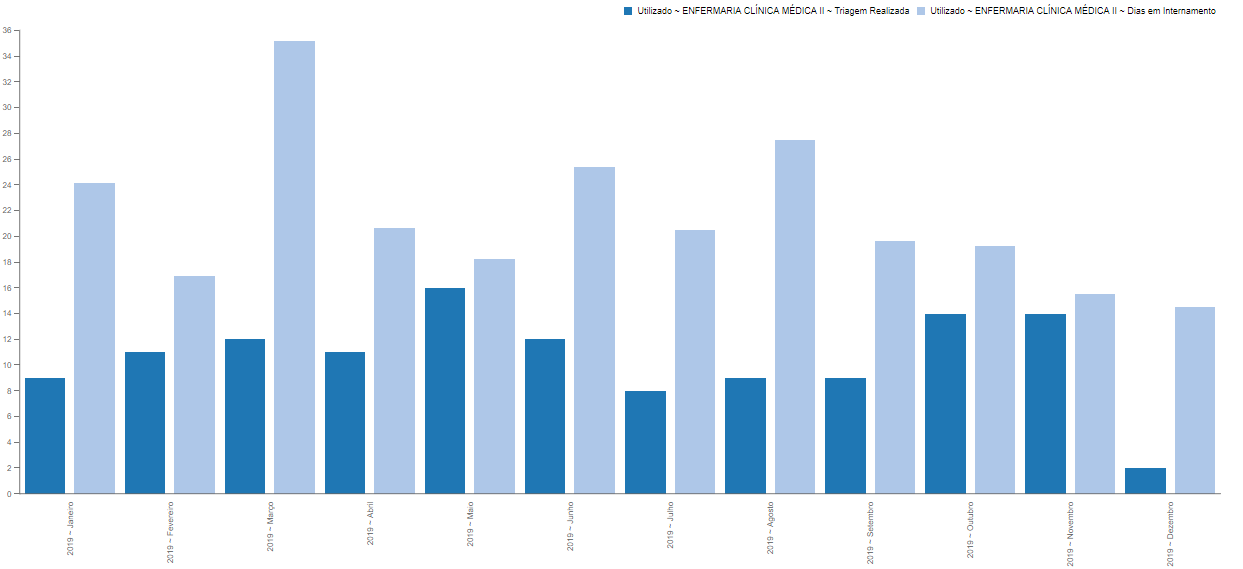
\includegraphics[scale=0.35]{Imagens/6.2.TotalUsoSuplementoMediaDeDiasInternadoEnfermariaMesBarra.png}
	\end{center}
	\legend{Fonte: Autor.}
\end{figure}

\subsection{Resultados}

Analisando os resultados da revisão sistemática e os resultados dos relatórios e \textit{dashboards} obtidos a partir do processamento dos dados da Unidade de Nutrição do HU, foi possível concluir que a solução de \textit{Business Intelligence} desenvolvida utilizou como fonte de dados planilhas eletrônicas e consultas ao sistema de administração hospitalar do HU, assim como nos estudos A4, A7, A10, A11, A12, A16 e A17 da revisão sistemática apresentados no \autoref{quadro_ImpactosPositivos}. Também como nos estudos A7 e A11, utilizou-se como estrutura de armazenamento de dados o modelo de \textit{Data Warehouse}. E para apresentação dos dados foi utilizado um \textit{plugin} da mesma forma que o estudo A2. Já para análise das informações foram utilizados \textit{dashboards} disponibilizados aos usuários por meio de aplicação web assim como nos estudos A1, A5, A10, A15 e A17.

O \textit{feedback} relatado até o momento pela Unidade de Nutrição do HU foi de um ganho de eficiência na geração dos dados e gráficos que regularmente são encaminhados aos gestores do hospital e perceptível ampliação do espectro de análise, uma vez que, os \textit{dashboards} comparam dados mensais e anuais, levando não apenas o detalhamento por enfermaria, mas permite a comparação da situação entre as várias enfermarias do hospital. É possível ainda estender a utilização da aplicação para outros períodos configurando tarefas, denominadas de \textit{jobs} no \textit{Pentaho Data Integration}, que podem ser agendadas para execução dinâmica do processo de ETL, importando outros arquivos de fontes de dados ou consultando o sistema de administração do hospital. A \autoref{fig_diagramaimplantacao} apresenta o diagrama de implantação, que provê uma representação gráfica dos dispositivos que devem estar envolvidos para execução da solução de BI. 

\begin{figure}[htb]
	\caption{\label{fig_diagramaimplantacao}Diagrama de Implantação.}
	\begin{center}
	    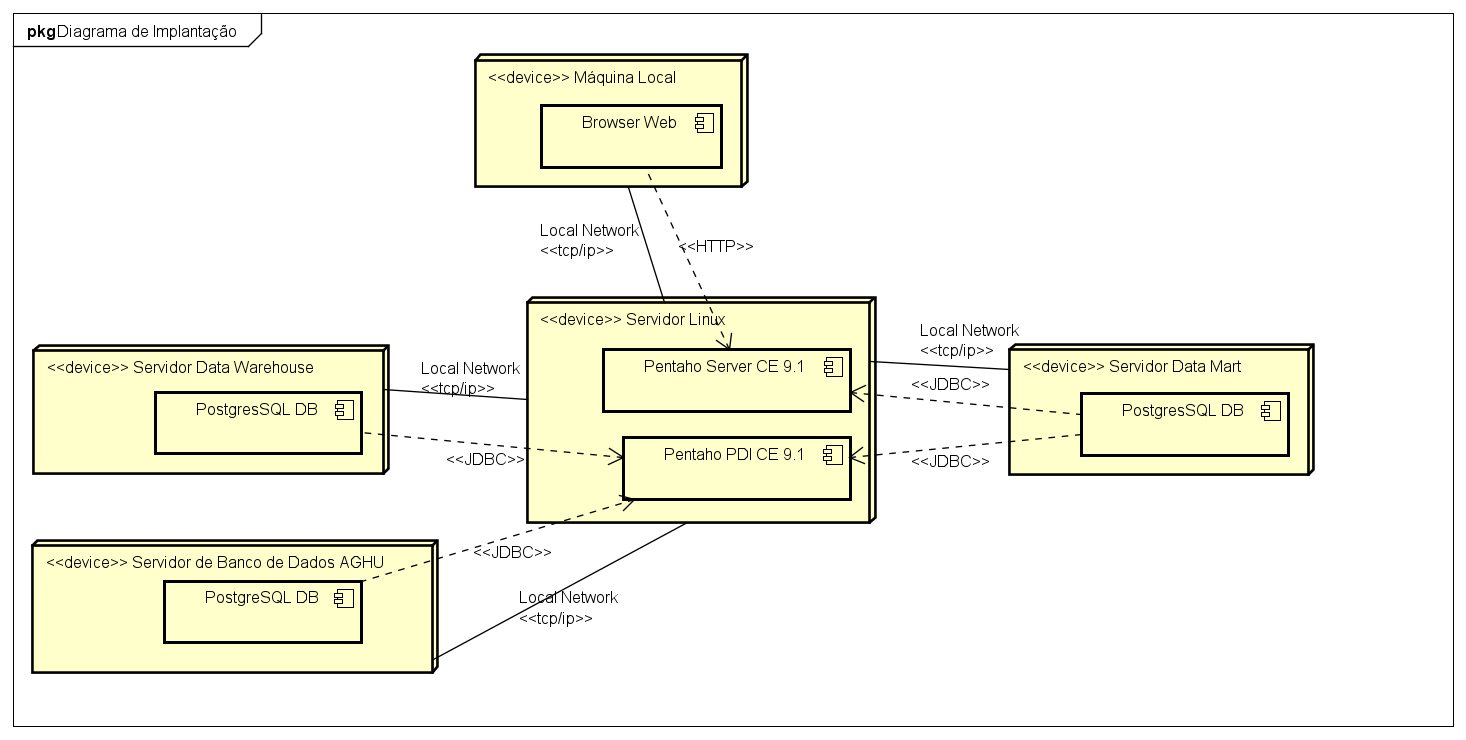
\includegraphics[scale=0.41]{Imagens/figura - diagrama de implantação.png}
	\end{center}
	\legend{Fonte: Autor.}
\end{figure}

Um dos pontos de maior dificuldade durante o projeto esteve no tratamento dos dados da planilha eletrônica, decorrente da falta de padronização na inserção de dados. Por se tratar de um documento de preenchimento aberto, existe pouco controle sobre como os dados são digitados, levando a uma grande discrepância entre o formato de preenchimento quando comparadas as diferentes enfermarias. Outro problema encontrado estava na solicitação de visualização de informações sobre dados que ainda não eram coletados, impossibilitando que alguns \textit{dashboads} fossem gerados.

O Hospital Universitário de Aracaju já dispõe de um sistema de informação nutricional em fase de homologação para a Unidade de Nutrição \cite{crisnaldo2020}. Existem expectativas para uso em um futuro próximo, permitindo que os dados possam ser consultados diretamente da base de dados do sistema, possibilitando que os processos de ETL sejam padronizados em agendamentos de \textit{jobs} no \textit{Pentaho Data Integration}. Sendo possível assim, ampliar a quantidade de indicadores mensurados, para que mais informações sejam analisadas, visando reduzir o desperdício de recursos e também o tempo de internação dos pacientes, assim como descritos nos estudos A8 e A17, que apontaram a melhora desses índices com base na tomada de decisão orientada aos dados dos \textit{dashboards}.

\section{Considerações finais do capítulo}
Neste capítulo foi apresentado o processo de construção do ambiente BI para a unidade de nutrição do HU detalhando aspectos técnicos e escopo do projeto. Foram também descritos o processo de ETL para monitoramento dos indicadores solicitados pela unidade de nutrição do hospital, a modelagem de um cubo lógico e o desenvolvimento de \textit{querys} de consulta que são utilizadas na plataforma Pentaho, bem como, a construção dos \textit{dashboards} para interpretação dos dados coletados pelo departamento. O próximo capítulo apresenta as considerações finais deste trabalho.


% ---
\chapter{Considerações Finais}
% ---
Este trabalho apresentou uma solução de \textit{Business Intelligence} para a Unidade de Nutrição Clínica do Hospital Universitário de Aracaju, transformando os dados gerados pela unidade em informação para apoiar a gestão do departamento na tomada de decisão gerencial.

O estado nutricional do paciente internado impacta diretamente na melhora ou piora da sua condição clínica. E mensurar, avaliar e melhorar os indicadores de qualidade do processo de terapia nutricional é imprescindível para melhorar o atendimento aos usuários do serviço de saúde hospitalar. O que consequentemente também melhora a qualidade de vida do paciente, ajudando a reduzir seu tempo de internação, reduzindo gastos hospitalares e possibilitando que os recursos sejam melhor aplicados. A solução de BI desenvolvida atua no processo de análise de dados da gestão do HU provendo \textit{dashboards} com indicadores calculados em diferentes dimensões ampliando o campo de alcance das informações.

O desenvolvimento da solução de BI foi apoiado por algumas etapas sendo que uma revisão sistemática foi realizada para extração de informações relevantes de trabalhos publicados em bases acadêmicas que tratam da aplicação de sistemas de apoio à decisão para nutrição em ambiente hospitalar. Ocorreram reuniões e visitas a Unidade de Nutrição do HU com o objetivo de elencar requisitos para desenvolvimento dos \textit{dashboards}.

Como \textit{feedback}, a Unidade de Nutrição do HU apontou satisfação e ganhos na produtividade, no que diz respeito a geração dos dados para posterior análise. As informações disponibilizadas se mostraram de grande utilidade para as nutricionistas do departamento, principalmente sobre os indicadores de dieta enteral, suplementação, estado nutricional e classificação de risco. Espera-se também que a utilização do BI no monitoramento dos indicadores de terapia nutricional contribua para a instituição, sendo uma fonte de informações confiáveis e eficazes para a tomada de decisão. O sistema BI proporciona análise analítica de informações para auxiliar a gestão hospitalar numa melhor condução da prestação dos serviços hospitalares.

Para trabalhos futuros, sugere-se avaliar o desempenho e a utilidade do ambiente BI no cumprimento das demandas de decisão da gestão da unidade, conectar o Sistema de Informação Nutricional que está em fase de homologação na unidade, em substituição ao atual modelo de registro de informações em planilhas eletrônicas, incluindo assim uma fonte de dados íntegra e atualizada do departamento, afim de responder com informações importantes no menor tempo possível, possibilitando a criação de tarefas de ETL agendadas para carga de informações no D\textit{ata Warehouse}.